
\documentclass[11pt]{article}


\usepackage{amssymb, amsmath, verbatim, amsthm,url, multirow,fullpage,mathtools}
\usepackage{longtable, rotating,makecell,array}
\usepackage[aligntableaux=top]{ytableau}


\setlength{\parindent}{0pt}
\setlength{\parskip}{1.5ex plus 0.5ex minus 0.2ex}


%***************************
%Frontmatter Table of contents
%***************************
% Annotations
%xypic packages
%WLD tkx program
%Useful numeric rings and fields
%Other useful mathematical operations and functions
%Equation display shortcuts
%Shortcuts for frequently used special characters
%Theorem environments
%***************************

%*****************
% Annotations
\usepackage{soul}
\usepackage[colorinlistoftodos,textsize=footnotesize]{todonotes}
\newcommand{\hlfix}[2]{\texthl{#1}\todo{#2}}
\newcommand{\hlnew}[2]{\texthl{#1}\todo[color=green!40]{#2}}
\newcommand{\note}{\todo[color=green!40]}
\newcommand{\newstart}{\note{The inserted text starts here}}
\newcommand{\newfinish}{\note{The inserted text finishes here}}
\setstcolor{red}
%***************************


%*****************
%xypic packages
\usepackage[all]{xy}
\xyoption{poly}
\xyoption{arc}
%*****************

%*****************
%%% WLD drawing and 2,6 shortcuts

\usetikzlibrary{decorations.pathmorphing,calc}
\usetikzlibrary{intersections}




\definecolor{light-gray}{gray}{0.6}


\tikzstyle{propagator}=[decorate,decoration={snake,amplitude=0.8mm}]
\tikzstyle{smallpropagator}=[decorate,decoration={snake,segment length=3mm,amplitude=0.5mm}]

% these two for drawing partial propagators
\tikzstyle{firstdash}=[dashed,line cap=round, dash pattern=on 2pt off 1pt]
\tikzstyle{seconddash}=[dashed,line cap=round, dash pattern=on 0.5pt off 1pt]

% vertices, radius
\newcommand{\drawWLD}[2]{

\pgfmathsetmacro{\n}{#1}
\pgfmathsetmacro{\radius}{#2}
\pgfmathsetmacro{\angle}{360/\n}
    \foreach \i in {1,2,...,\n} {
      \pgfmathsetmacro{\x}{\angle*\i}
        \draw[-,shorten >=-\radius*0.1 cm,shorten <=-\radius*0.1 cm]  (\x:\radius cm)-- (\x + \angle: \radius cm);
    }

\draw (\angle:\radius) node {$\bullet$};
}


% r, bumpr, s, bumps: r, s are start/end vertices, bumpr and bumps are how many steps to bump the start/end for multiple props on one edge
\newcommand{\drawprop}[4]{
\pgfmathsetmacro{\r}{#1}
\pgfmathsetmacro{\bumpr}{#2}
\pgfmathsetmacro{\s}{#3}
\pgfmathsetmacro{\bumps}{#4}
\pgfmathsetmacro{\perturbe}{\angle/\n}

\begin{scope}
\clip (\angle*\r:\radius) -- (\angle + \angle*\r:\radius) -- (\angle*\s:\radius) -- (\angle + \angle*\s:\radius) -- (\angle*\r:\radius);
\draw[propagator] (\angle*\r + \angle/2 + \bumpr*\perturbe:\radius) -- (\angle*\s + \angle/2 + \bumps*\perturbe:\radius);
\end{scope}
}

% for anything that requires modifying the propagator, e.g. colour, different amplitude,etc
% 5th argument should be {propagator,<other stuff>} or {smallpropagator,<otherstuff>} otherwise you'll get a straight line
\newcommand{\modifiedprop}[5]{
\pgfmathsetmacro{\r}{#1}
\pgfmathsetmacro{\bumpr}{#2}
\pgfmathsetmacro{\s}{#3}
\pgfmathsetmacro{\bumps}{#4}
\pgfmathsetmacro{\perturbe}{\angle/\n}

\begin{scope}
\clip (\angle*\r:\radius) -- (\angle + \angle*\r:\radius) -- (\angle*\s:\radius) -- (\angle + \angle*\s:\radius) -- (\angle*\r:\radius);
\draw[#5] (\angle*\r + \angle/2 + \bumpr*\perturbe:\radius) -- (\angle*\s + \angle/2 + \bumps*\perturbe:\radius);
\end{scope}
}


\newcommand{\boundaryprop}[4]{
\pgfmathsetmacro{\r}{#1}
\pgfmathsetmacro{\bumpr}{#2}
\pgfmathsetmacro{\s}{#3}
\pgfmathsetmacro{\perturbe}{\angle/\n}

\begin{scope}
\clip (\angle*\r:\radius) -- (\angle + \angle*\r:\radius) -- (\angle*\s - \angle:\radius) -- (\angle*\s:\radius) -- (\angle + \angle*\s:\radius) -- (\angle*\r:\radius);
\draw[#4] (\angle*\r + \angle/2 + \bumpr*\perturbe:\radius) -- (\angle*\s:\radius);
\end{scope}
	
}





\newcommand{\drawnumbers}{
  \foreach \i in {1,2,...,\n} {
  \pgfmathsetmacro{\x}{\angle*\i}
  \draw (\x:\radius*1.15) node {\footnotesize \i};
}
}




\newcommand{\boundA}[3]{
	\pgfmathsetmacro{\r}{#1}
	\pgfmathsetmacro{\bumpr}{#2}
	\pgfmathsetmacro{\destination}{#3}
	\pgfmathsetmacro{\perturbe}{\angle/\n}
	\path [name path=polyedge1] (\angle*\r:\radius) -- (\angle*\r + \angle:\radius);
	\path [name path=radius1] (0:0) -- (\angle*\r + \angle/2 + \bumpr*\perturbe:\radius);
	\draw[->,
	name intersections={of=polyedge1 and radius1,by=p},
	shorten >=\radius*0.1 cm] (p) ++(\angle*\r + \angle/2 + \bumpr*\perturbe:\radius*0.15) -- (\angle*\destination: \radius*1.15);

}



\newcommand{\boundB}[3]{
	\pgfmathsetmacro{\rangle}{#1*\angle + \angle/2 + #2*\angle/\n}
	\pgfmathsetmacro{\sangle}{#1*\angle + \angle/2 + #3*\angle/\n}


	\draw[->,shorten <=\radius*0.02cm,shorten >=\radius*0.05cm] (\rangle:\radius*1.05) -- (\sangle:\radius*1.05);

}



\newcommand{\makediag}[8]{
	\begin{tikzpicture}[rotate=60,baseline=(current bounding box.east)]
	\begin{scope}
	\drawWLD{6}{0.8}
	%\drawnumbers
	\drawprop{#1}{#2}{#3}{#4}
	\drawprop{#5}{#6}{#7}{#8}
	\end{scope}
	\end{tikzpicture}
}


%*****************

%*****************
%Useful numeric rings and fields
\newcommand{\Q}{\mathbb{Q}}
\newcommand{\Z}{\mathbb{Z}}
\newcommand{\C}{\mathbb{C}}
\newcommand{\R}{\mathbb{R}}
\newcommand{\N}{\mathbb{N}}
\newcommand{\RP}{\mathbb{R}\mathbb{P}}
\newcommand{\id}{\mathbb{I}}
\newcommand{\Gr}{\mathbb{G}_{\R, \geq 0}}
\newcommand{\Grtnn}{\mathbb{G}_{\R, +}}
\newcommand{\CW}{\overline{\mathcal{W}}} % CW complex of W(k,n)
\newcommand{\BW}{\widehat{\mathcal{W}}} % complex minus bald spots
%*****************

%*****************
%Other useful mathematical operations and functions
\newcommand{\D}{\partial}
\newcommand{\rk}{\textrm{rk}}
\newcommand{\spn}{\textrm{span }}
\newcommand{\rd}{\textrm{d}}
\newcommand{\Res}{\textrm{Res}}
%*****************

%*****************
%Equation display shortcuts
\def\ba #1\ea{\begin{align} #1 \end{align}}
\def\bas #1\eas{\begin{align*} #1 \end{align*}}
\def\bml #1\eml{\begin{multline} #1 \end{multline}}
\def\bmls #1\emls{\begin{multline*} #1 \end{multline*}}
%*****************


%*****************
%Shortcuts for frequently used special characters
\newcommand{\fB}{\mathfrak{B}}
\newcommand{\cP}{\mathcal{P}}
\newcommand{\fZ}{\mathfrak{Z}}
\newcommand{\cM}{\mathcal{M}}
\newcommand{\cA}{\mathcal{A}}
\newcommand{\cI}{\mathcal{I}}
\newcommand{\cC}{\mathcal{C}}
\newcommand{\cB}{\mathcal{B}}
\newcommand{\G}{\mathbb{G}}
\newcommand{\Prop}{\textrm{Prop}}
\newcommand{\cW}{\mathcal{W}}
\newcommand{\bM}{\mathbb{M}}
\newcommand{\cZ}{\mathcal{Z}}
\newcommand{\cY}{\mathcal{Y}}
\newcommand{\Dom}{\textrm{Dom}}
\newcommand{\detzr}[1] {\langle (\cZ_*^\mu|V_p)^{#1} \rangle}
\newcommand{\II}{\mathcal{I}}
\newcommand{\PP}{\mathcal{P}}
\newcommand{\BB}{\mathcal{B}}
\newcommand{\CS}{\mathcal{S}}
\newcommand{\interval}[2]{[\![#1,#2]\!]}
\newcommand{\gale}[1]{\preccurlyeq_{#1}}
\newcommand{\sgale}[1]{\prec_{#1}}
%*****************

%*****************
%Theorem environments
\newtheorem{thm}{Theorem}[section]
\newtheorem{conj}[thm]{Conjecture}
\newtheorem{lem}[thm]{Lemma}
\newtheorem{cor}[thm]{Corollary}
\newtheorem{prop}[thm]{Proposition}
\newtheorem{algorithm}[thm]{Algorithm}


\theoremstyle{remark}
\newtheorem{eg}[thm]{Example}
\newtheorem{claim}[thm]{Claim}

\theoremstyle{definition}
\newtheorem{dfn}[thm]{Definition}
\newtheorem{rmk}[thm]{Remark}
\newtheorem{ntn}[thm]{Notation}
%*****************


\begin{document}

This paper studies the combinatorics of Wilson Loop Diagrams.
\section{Wilson Loop diagrams}

What are Wilson loop diagrams and their integrals.

\begin{dfn}\label{WLdfn}
A Wilson loop diagram is given by the following data: a cyclicly ordered set $V$, along with a choice of first vertex, and $k$ pairs $\{p_r = (i_r, j_r)\}_{r=1}^k$ ordered such that $i_r +1 < j_r$. \end{dfn}

We depict this data as a convex polygon, with vertices labeled by $V$ (preserving the cyclic ordering), and $k$ wavy lines in the interior of the diagrams. We depict the choice of first vertex on $V$ by a $\bullet$. Note that the polygon gives the verices of $W$ a cyclic ordering, which the choice of first vertex gives it a compatible linear order. Both the cyclic and the linear order become the correct perspective at various points in this paper. The pair $p_r$ defines a wavy line from the $i_r^{th}$ edge (between $i_r$ and $i_r+1$) and the $j_r^{th}$ edge. These are called propagators.  The condition on $i_r$ and $j_r$ means that the propagator does not go between adjacent edges. Let $\cP = \{p_r\}_{r=1}^k$ be the set of propagators. Then we write \bas W = (\cP, V) \;.\eas

Often we take $V$ to be $[n]$, the cyclically ordered set of integers, $1 \ldots n$. In this case, we write $W = (\cP, n)$. We introduce some notation to speak of vertices supporting a propagator, and the set of propagators supported on a vertex set.

\begin{dfn} \label{VPropdfn}
Let $W = (\cP, n)$.
\begin{enumerate}
\item For $p \in \cP$, let $V_p = \{i_p, i_p+1, j_p, j_p+1\}$ be the set of vertices supporting $p$. Then, for $P \subseteq \cP$, the set $V_P = \cup_{p \in P} V_p$ is the vertex support of $P$.
\item For $V \subseteq [n]$, write $\Prop(V) = \{ p \in \cP | V_p \cap V \neq \emptyset \} $.
\item For $P \subseteq \cP$, define $F(P) = V(P^c)^c$ to be the set of vertices in $[n]$ that only support propagators in the set $P$.
\end{enumerate}
\end{dfn}

It is sometimes useful to discuss propagators in terms of the edges supporting them, rather than the vertices.

\begin{dfn}
The $i^{th}$ edge of $W$ is the edge of the external polygon that lies between the vertices $i$ and $i+1$.
\end{dfn}

In this manner, the propagator $p = (i, j)$ is supported by the $i^{th}$ and $j^{th}$ edges.

\begin{dfn}\label{admisdfn}
A Wilson loop diagram is admissible if \begin{enumerate}
\item $|V| \geq |\cP| + 4$
\item There does not exists a set of propagators, $P \subset \cP$ such that $|V(P)| < |P| + 3$.
\item There does not exist a pair of propagators, $p, q \subset \cP$ such that $i_p < i_q < j_p <j_q$.
\end{enumerate}
 \end{dfn}

The first conditions states that there are at least four more vertices than propagators in an admissible Wilson Loop Diagram. The second imposes an upper bound on how densely the propagators can be fitted in the diagram. The third ensures that ensures that no propagators cross in the interior of the diagram. In other words, a Wilson loop diagram, $(\cP, n)$ is admissible if and only if $n > \cP +4$, and has neither crossing propagators nor any pairs of propagators that start and end on the same pair of non-adjacent edges.

In what follows, we will talk about admissible Wilson Loop diagrams and subdiagrams thereof.

\begin{dfn} \label{subdiagramdfn}
Let $W = (\cP, n)$ be an admissible Wilson loop diagram. A subdiagram of $W$ is defined by a a subset of propagators of $W$. For $P \subset \cP$, write $W|_P = (P, V(P))$.
\end{dfn}
\note{Later I will also want a different kind of subobject, one with a subset of the propagators but where the vertex set contains $V(P)$ but may be larger (the most important instance being when it is $[n]$.)  This kind of subobject doesn't need a particular name, nor does it need to be defined up here, but I wanted to mention it so we have it in mind.}

Note that a subdiagram of an admissible diagram need not be admissible. In particular, the condition $|V(P)| > |P| +4$ need not hold.

There is one particular type subdiagram that deserves special attention.

\begin{dfn}
For $W$ an admissible diagram, $(P, V(P))$ is exact if $|V(P)| = |P| + 3$.
\end{dfn}

The exact subdiagrams define an equivalence relation amongst Wilson loop diagrams.

\begin{dfn}\label{equivdfn} \todo{I feel like I need some sort of uniqueness of partition result to even be able to define this well. Or something. Can we discuss?}
There is an equivalence relationship on the set of admissible Wilson loops diagrams generated by the following binary relation: $W = (\cP, n) \sim W'= (\cP', n)$ if
\begin{enumerate}
\item There exist two different exact subdiagrams, $(P, V(P))$ and $(P', V(P'))$ of $W$ and $W'$ respectively such that $V(P) =  V(P')$.
\item The complementary subdiagrams are identical: $(\cP \setminus P, V(P)^c) = (\cP' \setminus P', V(P')^c)$.
\end{enumerate}
\end{dfn}

\begin{eg}
Note that since this is an equivalence relation, we may find that two Wilson loop diagrams are equivalent, even if they do not have complements of (non-trivial) exact subdiagrams in common. Consider the following three Wilson loop diagrams,
\bas
W_1 = 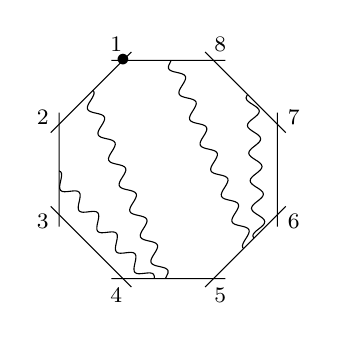
\begin{tikzpicture}[rotate=67.5,baseline=(current bounding box.east)]
	\begin{scope}
	\drawWLD{8}{1.5}
	\drawnumbers
	\drawprop{1}{0}{4}{0}
	\drawprop{2}{0}{4}{-1}
    \drawprop{5}{0}{8}{0}
    \drawprop{5}{1}{7}{0}
		\end{scope}
	\end{tikzpicture} \quad
W_2 = 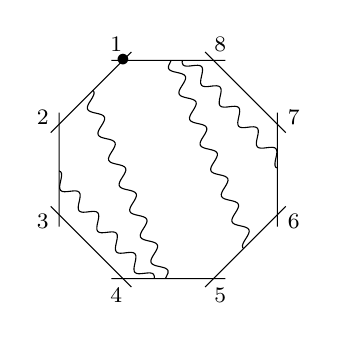
\begin{tikzpicture}[rotate=67.5,baseline=(current bounding box.east)]
	\begin{scope}
	\drawWLD{8}{1.5}
	\drawnumbers
	\drawprop{1}{0}{4}{0}
	\drawprop{2}{0}{4}{-1}
    \drawprop{5}{0}{8}{0}
    \drawprop{6}{0}{8}{-1}
		\end{scope}
	\end{tikzpicture} \quad
W_3 = 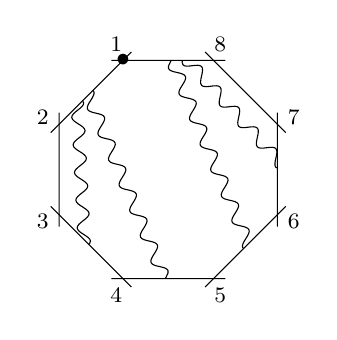
\begin{tikzpicture}[rotate=67.5,baseline=(current bounding box.east)]
	\begin{scope}
	\drawWLD{8}{1.5}
	\drawnumbers
	\drawprop{1}{0}{4}{0}
	\drawprop{1}{1}{3}{0}
    \drawprop{5}{0}{8}{0}
    \drawprop{6}{0}{8}{-1}
		\end{scope}
	\end{tikzpicture} .
\eas

The diagrams $W_1 \sim W_2$ because $(\{(5,8), (5,7), \{5,6,7,8,1\})$ and $(\{(5,8), (7,8), \{5,6,7,8,1\})$ are the corresponding differing subdiagrams. Furthermore, there is the equivalence $W_2 \sim W_3$ due to the exact subdiagrams $(\{(1,4), (3,4)\}, \{1,2,3,4,5\})$ and $(\{(1,4), (1,3)\}, \{1,2,3,4,5\})$. This forces an equivalence between $W_1$ and $W_3$, even though one cannot partition the propagators of each into a an exact subdiagram (that may vary between the diagrams) and a complement that is fixed.  \end{eg} 

\section{Wilson Loop diagrams as matroids}

In \cite{wilsonloop}, Amat and Agarwala show that admissible Wilson loop diagrams with $k$ propagators corresponds to positroids of rank $k$ (a matroid that can be represented by an element of $\Gr(k, n)$.)

\begin{thm}[\cite{wilsonloop}] An admissible Wilson loop diagram, $W =(\cP, n)$, defines a matroid with base set $[n]$. The independent sets are exactly those subsets $V \subseteq [n]$ such that $\not \exists U\subseteq V$ satisfying $|\Prop(U)|> |U|$. \label{thm:WLDmatroid}\end{thm}

This does not, however, show that the matroid associated to each Wilson loop diagram is unique. In fact, in \cite{wilsonloop}, the authors show that if two diagrams are equivalent then they define the same matroid [cite theorem here].

In the remainder of this section, we show that two admissible Wilson loop diagrams define the same matroid if an only if they are equivalent. Furthermore, we count the number of Wilson loop diagrams in each equivalence class. The first of these are done by considering Wilson loop diagrams as matroids. The second, by considering polygon partitions of Wilson Loop Diagrams.

To this end, we recall some definitions and go through a series of new intermediary steps.

First we recall a few facts about matroids, with particulars about those defined by Wilson loop diagrams.

\begin{dfn} For a Wilson Loop diagram $W = (\cP, [n])$, the associated matroid $M(W)$ can be defined by any of the following sets of subsets
\begin{enumerate}
\item An set $V \subseteq [n]$ is independent if there is no subset that supports fewer propagators than vertices of that subset: \bas \not \exists U \subseteq V \; \textrm{s.t. } |\Prop (U)| < |U|\;. \eas A basis of $W$ is any independent set, $B \subset [n]$ of size $|B| = |\cP|$.
\item The rank of a set $|V| \subset [n]$, is bounded above by $\rk(V) \leq \min\{ |V| , |\Prop(V)|\}$. If $V$ is an independent set, then $\rk(V) = |V|$. Furthermore, if $v \in [n]$, and $q \in \Prop(v)$, then for any $V \subset [n]$ such that $q \not \in \Prop(V)$, $\rk(V \cup v) = \rk(V) +1$. That is, adding a vertex that supports a new propagator to a set increases the rank of the set.
\item A circuit of a matroid is any set $C \subset [n]$ such that every proper subset $U \subsetneq C$ is independent. That is, $\rk(C) = |C|-1$. The union of circuits is called a cycle. If $C$ is a circuit of an admissible Wilson loop diagram, and $e \in C$, \bas |\Prop(C\setminus e))| \leq |C\setminus e| = \rk(C) \leq \min\{|C|, |\Prop(C\setminus e)|\}\;.\eas
    In other words, if $C$ is a circuit of a Wilson loop diagram, then \bas \rk(C) = |C|-1 = |\Prop(C)| \;. \eas
\item A flat, $F$, of a matroid is a set that is maximal for its rank. That is, for all $e \not \in F$ $\rk(F \cup e) = \rk(F) +1$. If $W$ is an admissible Wilson loop diagram, any group of propagators defines a flat, $F(P) = V(P^c)^c$, called a propagator flat. To see that this is flat, let $v \in V(P^c)$. We have that there is a $q \not \in P$ such that $q \in \Prop(v)$. Therefore, by the rank function, $\rk( F(P) \cup v))> \rk(F(P))$. Furthermore, in \cite{wilsonloops}, the authors show that if $F$ is a cyclic flat, then there is a $P \subset \cP$ such that $F = F(P)$.

\end{enumerate}
\end{dfn}

It is worth noting that it is not necessary to list all the flats in a matroid to defined it completely, only the cyclic flats, and those that are independent sets. Namely, if $F$ is a dependent flat, it contains a circuit. Let $C \subset F$ be the largest cycle contained in $F$. Then two things are true.

\begin{lem} Let $W$ be a Wilson loop diagram, and $F$ is a flat. Let $C \subset F$ be the largest cycle contained in $F$. Then the following is true:
\begin{enumerate}
\item $C = F(\Prop (C))$ is a cyclic flat.
\item $F \setminus C$ is an independent set. If $W$ does not contain any vertices of rank $0$, that is, all vertices support at least $1$ propagator, then $F \setminus C$ is an independent flat.
\end{enumerate}
\end{lem}

\begin{proof}
If $F$ is an independent flat, then $C = \emptyset$ and the statement is trivially true.

If $F$ is a dependent set, $F$ contains a circuit.

To see the first point, note that $\rk(C) = |\Prop(C)| \geq F(\Prop (C)|$.  For any $v\in C$ we have that $\Prop(v) \subset \Prop(C)$. This implies that $v \in F(\Prop(C))$. Therefore $C \subset F(\Prop(C))$. This implies that $|\Prop(C)| = F(\Prop (C)|$. Suppose there is a $v \in  F(\Prop(C)) \setminus C$. Let $B$ be an independent subset of $C$ of maximal rank. The set $B \cup v$ is dependent and therefore contains a circuit. Therefore, $C \cup b$ is a cycle, which is a contradiction to $C$ being the maximal cycle in $F$.

To see the second point, note that $F \setminus C$ is independent (as it contains no circuits). Furthermore, it is a flat. For any $e \not \in F$, $\rk (F \setminus C \cup e) = \rk (F\setminus C) +1$, since $F$ is a flat. For any $e \in C$,  if $\rk (F \setminus C \cup e) = \rk (F\setminus C)$, the set $F \setminus C \cup e$ is a dependent set. This occures either if $\rk{e} = 0$, or $F\setminus C \cup e$ contains a circuit of at least $2$ elements, which contradicts the hypothesis that $C$ is the largest cycle in $F$.
\end{proof}

Therefore, in the sequel, one only needs worry about cyclic and independent flats.

\begin{cor} \label{classifyflats}
If $F$ is a flat of a Wilson loop diagram, it can be written as the union of a cyclic propagato flat and an independent flat. \end{cor}

In particular, any propagator flat can be written as a union of a cyclic propagator flat and an independent flat.


Finally, we note the differences between subdiagrams of Wilson loop diagrams, and restrictions or contractions of the associated matroids.

Given any matroid, one may restrict it to a subset of the base set. The bases of the restricted matroid come from intersecting bases of the original with the subset. It is worth noting that a the matroid defined by a subdiagram is different from the restriction of the matroid of a Wilson loop diagram to a set of vertices.

\begin{dfn} \label{restrictiondfn}
For $W = (\cP, n)$, the restricted diagram, $W|_V$ is the matroid defined by only looking at the vertices $V \subset [n]$.
\end{dfn}

The key difference between a subdiagram and a restriction is that the propagator support function does not change in the case of restriction, while it may in the case of a subdiagram. In particular, for $v \in V$, $\Prop_W(v) = \Prop_{W|_V}(v)$, while $\Prop_{(P, V(P))} (v) = \Prop_W(v) \cap P$.

A subdiagram is more closely related to a contracted matroid.

\begin{lem} \label{contractsubdiaglem}
For $W = (\cP, [n])$, consider a subdiagram $(P^c, V(P^c))$. The complementary set of vertices is a propagator flat: $F(P) = V(P^c)^c$. If this has maximal rank, $\rk F(P) = |P|$, then the subdiagram defines the same matroid as is formed by contracting the original matroid by $F(P)$: \bas M((P^c, V(P^c))) = M(W)/ F(P) \;. \eas
\end{lem}

In the sequel, where it doesn't cause confusion, I conflate a Wilson loop diagram with the matroid it defines.

\subsection{Polygon partitions of Wilson loop diagrams}

In order to study exact Wilson loop diagrams, we further introduce the notion of a polygon partition of $W$.

\begin{dfn}
  Let $W = (\cP, n)$ be an admissible Wilson loop diagram.  The \emph{polygon partition} associated to $W$, denotes $\tau(W)$ is defined as follows.
  \begin{itemize}
  \item The vertices of $\tau(W)$ correspond to the edges of $W$.
  \item Labeling the vertices of $\tau(W)$ with the edge number of $W$gives a cyclic order to the vertices. Connecting consecutive vertices gives a graph theoretic cycle called the polygon of $\tau(W)$.
  \item Each propagator of $W$ defines a chord edge of $\tau(W)$ for each propagator of $W$.  If $p= (i,j) \in \cP$, it defines a chord connecting the verices $i$ and $j$
  \end{itemize}
\end{dfn}

\begin{lem}\label{tausimpleplanarlem}
If $W = (\cP, n)$ is an admissible Wilson loop diagram, $\tau(W)$ is a simple planar graph wihose outer face is a cycle. It is embedded such that the vertices all like on this infinite face. These vertices are cyclically ordered, with a coice of first vertex, giving it an additional compatible linear order.
\end{lem}

\begin{proof}
Since the vertices of $\tau(W)$ are labeled by the edges of $W$, which are cyclically ordered, this gives an ordering to the vertices. Furthermore, since the outer polygon of $W$ is a cycle, the outer face of $\tau(W)$ is also a cycle. Since $W$ is admissible, no pairs of propagators cross. Thereofore, it is a planar embedding. There are no propagators $p = (i, i+1)$. Therefore, there is exactly one edge connecting any two adjacent edges of $\tau(W)$. Similarly, there are not two propagators such that both $p$ and $q$ start and end at the edges $i$ and $j$. Therefore, no other two vertices of $\tau(W)$ can be connected by more than one edge. Finally, the embedding of $\tau(W)$ is induced from embedding of the graph $W$.
 \end{proof}

\begin{comment}
\hlfix{For an admissible $W$ no propagators cross and so no chord edges of $\tau(W)$ cross.  Thus, in graph theoretic language, we can view $\tau(W)$ as a planar embedding of a
graph with no cut vertices, where all vertices lie on the infinite face, along with a distinguished start vertex and direction around the infinite face.  From this viewpoint the polygon of $tau(W)$ is the boundary of the infinite face.}{I've smushed this together a bit in the prev. lem. Tell me if I've missed anything. Its a lemma for emphasis, not difficulty}
\end{comment}

***draw some examples***

A planar embedding of a graph is a \emph{triangulation} if all faces, except possibly the infinite, face are triangles.

\begin{dfn}
  Let $W$ be an admissible Wilson loop diagram and $\tau(W)$ its polygon partition. A \emph{triangulated piece} of $\tau(W)$ is a 2-connected subgraph of $\tau(W)$ which is a triangulation. We will take the convention that a subgraph consisting of a single chord edge is called a \emph{trivial} triangulated piece.
\end{dfn}

A decomposition of a polygon partition $\tau(W)$ is a set of 2-connected induced subgraphs of $\tau(W)$ which partition the edges of $\tau(W)$.

\begin{lem} \label{decompositionlem}
  For $W$ an admissible Wilson loop diagram, the polygon partition $\tau(W)$ has a unique decomposition into maximal triangulated pieces, and edges in the polygon of $\tau(W)$.
\end{lem}

***draw an example***

\begin{proof}
We begin by giving an algorithm for the decomposition, then prove its uniqueness. Let $W = (\cP, n)$, with $|\cP| = k$.

Let $T(W)$ be a the dual graph of $\tau(W)$ with the vertex corresponding the to the infinite face split. In other words, place a vertex on each finite face of $\tau(W)$. These vertices are connected if there is a chord edge separating the edges. Furthermore, if the face is bounded by an edge of the polygonal cycle of $\tau(W)$, the corresponding vertex gets a leaf edge for each such boundary. Since, by Lemma \ref{tausimpleplanarlem}, $\tau(W)$ is a simple planar graph, $T(W)$ is an uniquely defined graph.

We claim that $T(W)$ is a tree. Since $\tau(W)$ is a planar graph with $k$ chord edges and no internal vertices, there are $k+1$ internal faces of $\tau(W)$. Each of these internal faces correspond to a vertex of $T(W)$, and there are $n$ vertices of $T(W)$ from the splitting of the dual graph, we see that $T(W)$ has $n+k+1$ vertices. On the other hand, $T(W)$ has $n+k$ edges, corresponding to the $n +k$edts of $\tau(W)$. Therefore, $T(W)$is a tree.

By construction, each face of $\tau(W)$ is a polygon. Therefore, each vertex of $T(W)$ is at least 3 valent (one for each edge of the polygon). If split each vertex of $T(W)$ if it is strictly greater than $3$ valent. (In other words, we fail to split exactly when the face is a triangle). The connected components of $T(W)$ correspond to the decomposition of $\tau(W)$ into maximal triangulated pieces and edges orinignaly in the polygon of $\tau(W)$.  Let $f$ be the forest thus obtained. The vertices of $f$ either have valence 1, (if they correspond leaf vertices) or 3,  (if they correspond to triangulated faces). Subtrees with no trivalent vertices correspond to either edges in the polygon of $\tau(W)$, if they were originally leaves of $T(W)$, or to maximal trivial triangulations. Splitting at all the faces that are not triangles ensures maximality of the decomposition. If the splitting were not maximal, then one could add a triangle to a connected component of the splitting, but this would imply that that splitting happened at a valence $3$ vertex.

To see uniqueness, consider a different maximal decomposition of $\tau(W)$. This induces a splitting on $T(W)$, where each connected component of the new decomposition corresponds to a subtree. Call this forest $f'$. Since $f' \neq f$, there are two trees, $t$ and $t'$ in $f$ and $f'$ that are distinct, but share at least one edge of $T(W)$. Since $f'$ is also maximal, $t'$ is not a subtree of $t$. Therefore, the edges of $t'$ can be found in at least two trees in the forest $f$. In particular, there is a vertex $v$ in $t'$ that corresponds to a split vertex of $T(W)$ in the original decomposition. This implies that $v$ has valence greater than $3$ in $T(W)$, and thus the corresonding face of $\tau(W)$ is not a triangle. In otherwords, the decomposition corresponding to $f'$ is not a triangulation. \note{This is a variant of what you wrote in the e-mail. Let me know if you like it.}
\end{proof}

\begin{cor} \label{maxtriangdisjointcor}
Given a maximal decomposition of $\tau(W)$, the maximal triangulated pieces are edge disjoint.
\end{cor}

\begin{proof}
If two maximal triangulated pieces were not disjoint, then one could take the union of the edges involved to get a larger triangulated piece. \note{Is it this simple? This is a variant of the proof on propagators}
\end{proof}

\subsection{Exact subdiagrams}

It has been proved that if two Wilson loop diagrams are equivalent, then the define the same matroid in \cite{wilsonloops}. In this section, we prove that two Wilson loop diagrams are equivalent if and only if they define the same matroid. Furthermore, we count the admissible elements of each equivalence class.

We begin by relating triangulations and exact subdiagrams.

\begin{lem}\label{lem triang to exact}
  Let $W$ be an admissible Wilson loop diagram and $\tau(W)$ its polygon partition.  The triangulated pieces of $\tau(W)$ correspond to the exact subdiagrams of $W$.
\end{lem}

\begin{proof}
  Let us first record a few standard facts about polygon triangulations (that is about triangulations with all vertices on the outer face).  If such a triangulation has $n$ vertices then it has $n$ edges on the polygon (that is on the outer face) and $n-3$ edges which are not.  No planar graph with the same vertices and the same outer face can have more edges than the triangulation and every such simple graph with $n-3$ edges off the outer face is a triangulation.

  Since $W$ is admissible, by lemma \ref{} $\tau(W)$ is a simple graph. Furthermore, $t$ is not all of $\tau(W)$.
  Let $t$ be a triangulated piece of the decomposition of $\tau(W)$ given in Lemma \ref{decomplem} and suppose $t$ has $n>2$ vertices.  We want to count how many edges of $t$ are not on the outer face of $\tau(W)$.  Consider the intersection of $t$ with the outer face of $\tau(W)$.  This is a possibly disconnected subgraph of the polygon of $\tau(W)$ with $n$ vertices, call it $S$.  Let $k$ be the number of connected components of $S$.   To join the components $S$ must have $k$ edges not in the outer face of $\tau(W)$.  Furthermore $t$ has $n-3$ edges not in its outer face and so also not in the outer face of $\tau(W)$.  Thus there are $n-3+k$ edges of $t$ not in the outer face of $\tau(W)$.

  Each of these $n-3-k$ internal edges correspond to propagators in $W$, call this set $P$.  Next we count the size of $V(P)$.  Each of the $n$ vertices in the outer face of $t$ corresponds to an edge of $W$. These $n$ edges define $k$ connected compnents of the outer polygon of $W$. Thus the set$V(P)$ has $n+k$ vertices.  In other words, \bas |V(P)| = n+k = |P| -3\;.\eas

If $n=2$, then $t$ has two connected componenents. Therefore, $t$ corresponds to a propagator that connects two non-adjacent edges. Therefore, the trivial triangulation is a trivial exact subdiagram.

  Conversely if we have an exact subdiagram $(P, V(P))$ of $W = (\cP, n)$ supported on $|V(P)| = |P|+3$ vertices. Let $|P| = k>1$ and $k+3 = m$. Suppose the set $V(P)$ defines $c$ disjoint cyclic intervals of $[n]$. Then the corresponding subgraph of $\tau(W)$ has $m-c$ vertices. Call it $t$. If $t$ were a triangulated component, $t$ would have $k -c$ internal edges.

  The graph $t$ has $k$ edges that come from propagators, and $m - 2c$ edges that come from the boundary polygon of $\tau(W)$. Since $t$ has $m-c$ vertices, it has $m-c$ external edges, of which $c$ come from propagators. Therefore, of the $k$ edges of $t$ that come from propagators, $k-c$ are internal to the connected component. Therefore, this is triangulated.

  If $k=1$, and $(P, V(P))$ is a trivially exact subdiagram. Then $t$ is an edge internal to $\tau(W)$ connecting two boundary edges, which, by definition is a triangulation.


%  The statement of the lemma then follows form the fact that inclusion is preserved under $\tau$ and so maximality also corresponds under $\tau$.
\end{proof}

Next, we prove a few theorems about matroidal properties of exact subdiagrams.

\begin{thm} \label{exactcircuitlem}
Let $(P, V(P))$ be a subdiagram of $W= (\cP, [n])$. This is an exact subdiagram if and only if it defines a uniform matroid of rank $|P|$.
\end{thm}

\begin{proof}
A uniform matroid of rank $r$ is one in which any set of size $ \leq r$ is independent. A circuit of rank $m$ is a set $C$ of rank $m$ and size $m+1$ such that every proper subset of $C$ is independent. I.e., \emph{a circuit is a minimal dependent set.} In other words, a matroid of rank $r$ is uniform if and only if all circuits have rank $r$. If $C$ is a circuit, then $|C| = r+1$.

We prove the following claim: The set $V(P)$ contains no circuits, $C$, such that  $\rk C< |P|$ in $(P, V(P))$. Since the $V(P) = |P|+3$, $\rk V(P) \leq |P|$. This implies that all circuits $C$ of $(P, V(P))$ are of maximal rank, as desired.

Consider a subdiagram $(P, V(P))$ of $W$. Suppose there is a circuit, $C \subset V(P)$ such that $\rk C = |\Prop (C) | = m < |P|$. The size of the complement of $C$ is $|V(P) \setminus C| = |V(P)| -(m+1)$. However, since $C$ does not contain any propagators outside of $\Prop (C)$, the set $V(P \setminus \Prop(C)) \subset V(P )\setminus C$. In otherwords, there are $|P| - m$ propagators supported on (at most) $|V(P)|-m -1$ vertices: \bas |V(P \setminus \Prop (C))| \leq |V(P)| - m-1\;. \eas Since $W$ is an admissible Wilson loop diagram, the subdiagram $(P, V(P))$ satisfies $|R| +3 \leq |V(R)|$ for all $R \subset P$.  This gives \bas |P| - m +3 \leq V(P \setminus \Prop(C))\;. \eas These two inequalities are compatible if and only if \bas |P| +3 < |V(P)| \;. \eas

In other words, the matroid associated to thet subdiagram $(P, V(P))$ is not uniform if and only if $(P, V(P))$ is not exact.
\end{proof}

In \cite{wilsonloops}, the authors show that all exact Wislon loop diagrams correspond to positroids. That is, they correspond to matroids that can be represented by elements of the positive Grassmannians $\Gr(|\cP|, |V|)$.

\begin{dfn}
Given a Wilson loop diagram $W$, define the positroid cell associated to a Wislon loop diagram, $\Sigma(W)$, to be the cell in the CW complex on $\Gr(|\cP|, |V|)$ defined by the realizations of $W$ that lie in $\Gr(|\cP|, |V|)$.
\end{dfn}

With this definition in mind, we have the following corrolary:

\begin{cor}
Let $(P, V(P))$ be an exact subdiagram of $W$. The matroid associated to this subdiagram corresponds to the top dimensional cell in $\Gr(|P|, |V(P)|)$.
\end{cor}

\begin{proof}
The unique top dimensional cell of $\Gr(|P|, |V(P)|)$ is defined by all points in $\Gr(|P|, |V(P)|)$ such that all Plucker coordinates are strictly greater than $0$. Since $(P, V(P))$ is an exact subdiagram, this all $|P| \times |P|$ minors are non-zero. Intersecting these with the cases with the positive Grassmannians demands that all minors be strictly positive.
\end{proof}

Since the matroid defined by the subdiagram $(P , V(P))$ is not the same as the matroid associated to $W_{V(P)}$, one cannot say that the $W_{V(P)}$ is a uniform matroid. In fact, for any subset $U \subset V(P)$, $\rk_{W_{V(P)}}(U) \geq \rk_{(P , V(P))}(U)$. This is because adding propagators to vertices can only increase the rank. In particular this implies that, for any subset $U \subset V(P)$, if $|U| \leq |P|$, then $U$ is independent in both the restricted matroid $W_{V(P)}$, and the original, $W$.

To avoid the issue of exact diagrams being subdiagrams of other exact subdiagrams (for instance, any subdiagram $(q, V_q)$, for $q \in \cP$ is exact), I introduce a definition.

\begin{dfn}
We say $(P, V(P))$ is a maximal exact subdiagram of $W$ if there is not other exact subdiagram $(Q, V(Q))$ containing it.
\end{dfn}

Therefore, in keeping with Lemma \ref{lem triang to exact}, maximal exact subdiagrams of $W$ correspond to maximal triangular components of $\tau(W)$. In what follows, maximal exact subdiagrams/ maximal triangulations play a significant role. First, we show that maximal exact subdiagrams of an admissible Wilson loop diagram are disjoint.

\begin{cor} \label{uniqueproppartitioncor}
For $W = (\cP, n)$ can be uniquely decomposed into maximal exact subdiagrams. These subdiagrams maximal subdiagrams partition $\cP$.
\end{cor}

\begin{proof}
This is a corollary to Lemma \ref{decompositionlem}, that gives a unique decomposition of polygon partitions, $\tau(W)$,  into maximal triangulated pieces, and Lemma \ref{lem triang to exact}, which gives a correspondence between triangulated components and exact subdiagrams. Futhermore, corrollary \ref{maxtriangdisjointcor} shows that the maximal triangulations are edge disjoint, and thus the propagators defining maximal exact subsets are also disjoint. Combining this with the fact that by construction, the decomposition of $\tau(W)$ accounts for all chord edges, gives the desired unique partition of propagators.
\end{proof}

Finally, we discuss some flats formed by the complement of the propagators defining an exact subdiagram.

\begin{lem} \label{maxexactcomplementrank}
Let $W = (\cP, n)$ be a Wilson loop diagram, and $(P, V(P))$ an exact subdiagram with $P \subsetneq \cP$. Then the set $V(P)^c = F(P^c)$ is a propagator flat of maximal rank  \bas \rk F(P^c) = |P^c| \;. \eas If $(P, V(P))$ is maximal, then $F(P^c)$ is cyclic.
\end{lem}

\begin{proof}
By construction, $V(P)^c$ is a propagator flat. Furthermore, it is not empty. In particular, since $(P, V(P))$ is an exact subdiagram, the vertices $V(P)$ cannot support a larger set of propagators (otherwise $W$ would no longer be admissible). Therefore, since $P \subsetneq \cP$, $V(P)^c = F(P^c)$ is not an empty set.

Notice that $n= |V(P)| + |F(P^c)| \geq |P| + |P^c| +4$, and $|V(P)| = |P| +3$. Therefore \bas |F(P^c)| > |P^c| \;.\eas In other words, $F(P^c)$ is a dependent flat. By corollary \ref{classifyflats} $F(P^c)$ is the union of a cyclic flat and an independent flat.

Let $(P, V(P))$ be maximal exact subdiagram. Suppose $F(P^c) = C \cup F$, where $C$ is the largest cyclic flat contained in $F(P^c)$ and $F$ is a non-empty independent set. Since $C = F(\Prop(C))$, we can write $V(Q)^c = F(\Prop(C))$, with \ba Q = (\Prop(C))^c \label{Qdef}\;. \ea Furthermore, \ba \rk(F) = |F| \leq \rk(F(P^c)) - \rk(C)  \leq |P^c| - \rk(C) \;. \label{increasingrank}\ea The first equality comes from the fact that $F$ is an independent set. Combining \eqref{Qdef} and \eqref{increasingrank} gives \ba |P| + |F| \leq |P| + |P^c| - \rk(C) = |Q| \;. \label{Qsizebound}\ea Furthermore, since $V(Q) = F \cup V(P)$, we may write  \ba |V(Q)| = |F| + |V(P)| = |F| + |P| +3 \label{VQsize} \;.\ea Combining this with \eqref{Qsizebound} gives $|V(Q)| - 3 \leq |Q|$. That is, either $W$ was not admissible, or $(P,V(P))$ was not a maximal exact subdiagram. In otherwords, $F$ cannot be non-empty, proving that $F(P^c)$ is a cyclic flat, and therefore of maximal rank.

Let $(Q, V(Q))$ be an exact subdiagram that is not maximal, with $Q \subset P$ defining he maximal exact subdiagram above. Then by lemma \ref{??} $|V(P)| = |V(Q)| + |P \setminus Q|$. Let $F(P^c)$ be the cyclic set defined as the complement of $V(P)$. Then $V(Q)^c = F(P^c) \cup F$, where $F$ is an independent set of size $|P \setminus Q|$ and with $(P \setminus Q) \subset \Prop (F)$. Therefore, $\rk (F) = |Q^c|$.
\end{proof}


In other words, by Lemma \ref{contractsubdiaglem}a maximally exact subdiagram $(P, V(P))$  can be written as a contraction by the complementary propagator flat: \bas (P, V(P)) = W/F(P^c) \;.\eas

Now I am ready to prove the main theorem of this section.

\begin{thm}
Let $W= (\cP, [n])$ and $W'= (\cP', [n])$ be two Wilson Loop diagrams. They define the same matroid if and only if $W \sim W'$.
\end{thm}

\begin{proof}
One direction has been proved in previous work, but we give a different proof here to be consistent with the method of this document.

Assume that $W$ and $W'$ are equivalent. Without loss of generality, write $W = (P \cup R, [n])$ and $W' = (P \cup R', [n])$, where $P \subset \cP \cap \cP'$ and $(R, V(R))$ and $(R', V(R'))$ are two maximally exact subdiagrams, with $R \neq R'$, but $V(R) = V(R')$. If this is not the case, one may always find a family of diagram, $\{W_i\}$ satisfying this condition and forming a transitive chain connecting $W$ to $W'$ in the equivalence class.

Let $U \subset V(R)$ be any subset of size $|U| = |R|$. The set $U$ is independent in the subdiagram $(R, V(R))$, and thus in $W$. The complementary set $F(P)$ is a flat of maximal rank by lemma \ref{maxexactcomplementrank} ($\rk(F(P)) = |P|$). Let $B \subset F(P)$ be a maximal indpendent set ($\rk B = |P|$) in $F(P)$. Since $F(P)$ is a flat, adding any element of $V(R)$ to $B$ increases the rank. Therefore, any basis of $W$ can be written as $B \cup U$. However, since $F(P)$ is common to both $W$ and $W'$, and $V(R) = V(R')$, any any basis of $W'$ can also be written $B \cup U$. Thus both matroids have the same bases sets, proving that they are the same.

For the converse, assume that the matroids associated to $W$ and $W'$ are the same: $M(W) = M(W')= M$. Let $\{(P_i, V(P_i)\}_{i=1}^k$ and $\{(P'_i, V(P'_i)\}_{i=1}^l$ be the sets of maximally exact subdiagrams of $W$ and $W'$. Write $F_i = F(P_i)$ and $F'_i = F(P^{'c}_i)$ to be the complementary cyclic flats. By Lemma \ref{??} $M/F_i$ is a uniform matroid. Thereofore, $k = l$, and we may write $V(P_i) = V(P'_i)$.

Reorganize the vertex sets as follows: \ba \cup_{P_i \neq P_i'} V(P_i) = V(\cup_{P_i \neq P'_i} P_i)  \label{vertexsets}\; .\ea Since maximal exact subdiagrams partition $\cP$, by Lemma \ref{uniqueproppartitioncor}, write $cup_{i = 1}^k P_i = \cup_{i = 1}^k P'_i = \cP$. Then equation \eqref{vertexsets} becomes \bas \cap_{P_i \neq P_i'} (F(P_i^c))^c = F(\cup_{P_j = P'_j} P_j)^c \;.\eas These flats may, of course, be empty.

Thus, we have partitioned the vertices of $W$ and $W'$ into a single set that supports a union of maximal exact subdiagrams whose propagators between $W$ and $W'$, and the complementary propagator flats that support the propagators in common between $W$ and $W'$. As mentioned above, the latter may be empty.

Define a family of Wilson loop diagrams, $W_0$ to $W_k$ defined such that $W_0 = W$ and $W_i$ is derived from $W_{i-1}$ by replacing the propagator set $P_i$ with $P'_i$. In this manner, $W' = W_k$ and $W_i \sim W_{i+1}$, making $W \sim W'$.
\end{proof}

Since there is a unique way to decompose $W$ into maximal exact subdiagrams, it is logical to ask how many diagrams there are in an equivalence class. It is a classical fact the the number of triangulations of an $n$-gon is the $n-2$ Catalan number, namely $\frac{1}{n-1}\binom{2(n-2)}{n-2}$.  Thus we can count the number of equivalent diagrams.

\begin{cor}
  Let $W$ be an admissible Wilson loop diagram where the sizes of the supports of the maximal connected exact subdiagrams are $n_1, n_2, \ldots, n_j$.  Then the number of admissible Wilson loop diagrams equivalent to $W$ (including $W$ itself) is
  \[
  \prod_{i=1}^{j} \frac{1}{n_i-1}\binom{2(n_i-2)}{n_i-2}
  \]
\end{cor}


\begin{comment}
\subsection{Counting exact subdiagrams}


\begin{dfn}
  Say two admissible Wilson loop diagrams $W_1$ and $W_2$ are \emph{triangulation-equivalent} if there is a bijection $\alpha$ between the set of triangulated pieces in the decomposition of $\tau(W_1)$ and the set of triangulated pieces in the decomposition of $\tau(W_2)$, where $t$ and $\alpha(t)$ have the same vertex set for all triangulated pieces $t$ of $\tau(W_1)$.
\end{dfn}

***draw an example***

\begin{thm}
  Two admissible Wilson loop diagrams have the same matroid iff they are triangulation equivalent
\end{thm}

Again do I want matroid or positroid in this theorem?

\begin{proof}
  By Lemma~\ref{lem triang to exact} two admissible Wilson loop diagrams are triangulation equivalent iff their decompositions into maximal connected exact subdiagrams have matching supports, that is if they are equivalent.
  Theorem~\ref{thm orig equiv} then gives the result.
\end{proof}



\end{comment}

\section{Geometry of Wilson Loop diagram}
Since Wilson loop diagrams correspond to positroids, it is natural to understand the subspace of $\Gr(|\cP|, n)$ they define.

Talk about Grassmann Necklaces and how it defines a cell in a CW complex of $\Gr(k,n)$. Also talk about how this is exactly all the non-negative matrices that represent a particular positroid.

Also talk about Le diagrams.

\subsection{From Wilson Loop diagrams to Grassmann Necklaces}

Here, we give an algorithm for passing from Wilson loop diagrams to Grassmann Necklaces.

Let $\interval{1}{n}$ denote the set of integers $\{1,2, \dots, n\}$, and $\binom{[n]}{k}$ the set of all $k$-subsets of $\interval{1}{n}$.  For each $j \in \interval{1}{n}$, we can define a total order $\leq_j$ on the interval $\interval{1}{n}$ by
\[ j <_j j+1 <_j \dots <_j n <_j 1 \dots <_j j-1.\]
This in turn induces a total order on $\binom{[n]}{k}$, namely the lexicographic order with respect to $<_j$.  It also induces a separate partial order $\gale{j}$ on $\binom{[n]}{k}$ (the \textit{Gale order}), which is defined as follows: if $A = [a_1 <_j a_2 <_j \dots <_j a_k]$,  $B = [b_1 <_j b_2 <_j \dots <_j b_k] \in \binom{[n]}{k}$, then
\[A \gale{j} B \text{ if and only if } a_r \leq_j b_r \text{ for all }1 \leq r \leq k.\]
For example, in $\binom{[6]}{3}$ we have $[2,5,6]\gale{2} [2,6,1]$ but $[2,5,6]\not\gale{2}[3,4,6]$.


\begin{dfn}\label{def:grassmann necklace}
A Grassmann necklace of type $(k,n)$ is a sequence $\II = (I_1, \dots, I_n)$ of $n$ elements $I_i \in \binom{[n]}{k}$, such that
\begin{itemize}
\item if $i \in I_i$, then $I_{i+1} = \big(I_i \backslash \{i\}\big) \cup \{j\}$ for some $j \in \interval{1}{n}$.
\item if $i \not\in I_i$, then $I_{i+1} = I_i$.
\end{itemize}
\end{dfn}

By [ref], the Grassmann necklaces of type $(k,n)$ are in 1-1 correspondence with the positroid cells in $Gr(k,n)^{tnn}$.  Further, if $\II$ is the Grassmann necklace associated to a cell $\PP$, then the bases of $\PP$ can be computed using the Gale order $\gale{i}$ for each $i \in \interval{1}{n}$:
\[\BB(\PP) = \left\{J \in \binom{[n]}{k}\ :\ I_i \gale{i} J \ \forall i \in \interval{1}{n}\right\}.\]
We now describe an algorithm that, when applied to an admissible Wilson loop diagram, produces exactly the Grassmann necklace of the corresponding positroid.

\begin{algorithm}\label{alg:put GN on WLD}
Let $W$ be a Wilson loop diagram with $n$ vertices.  Note that whenever the algorithm below refers to the ``rightmost'' propagator supported on a vertex $i$, we mean the rightmost from the point of view of standing in the middle of the diagram and looking directly at $i$.

\begin{enumerate}
\item Fix a vertex $s \in \interval{1}{n}$, and set $i:=s$.
\begin{enumerate}
\item \textbf{Step $i$ for vertex $s$}: If there is at least one propagator in the current diagram supported on $i$, add the label $i$ to the edge $(s,s+1)$ and delete the rightmost propagator supported on $i$; otherwise do nothing.
\item If there are no propagators left in the diagram at this point, go to (2) below.
\item Otherwise, increment $i$ by 1 and repeat from (a).
\end{enumerate}
\item Replace all propagators in the diagram, and repeat from (1) for a new vertex $s$.  Continue until the algorithm has been applied to all vertices.
\end{enumerate}
\end{algorithm}


\begin{prop}\label{res:alg k labels}
If $W$ is an admissible Wilson loop diagram, then Algorithm~\ref{alg:put GN on WLD} puts exactly $k$ distinct labels on each edge.
\end{prop}
\begin{proof}
It is enough to show that the algorithm terminates in at most $n$ steps for each vertex.  Suppose this doesn't happen, i.e. there is a propagator $P$ which survives the first $n$ steps of the algorithm for some starting vertex $s$.  We will show that this always gives a contradiction in an admissible diagram by constructing an inductive sequence of propagators on strictly decreasing regions of the diagram.

Rotating and cyclically renumbering if necessary, we can assume that $s=1$ and that $P$ is supported on $(a,a+1,b,b+1)$ with $1 \leq a < b$.  Since $P$ is not removed at step $b+1$, there is another propagator $p_1$ to its right which is also supported on $b+1$: see Figure~\ref{fig:base step of alg induction}.

\begin{figure}
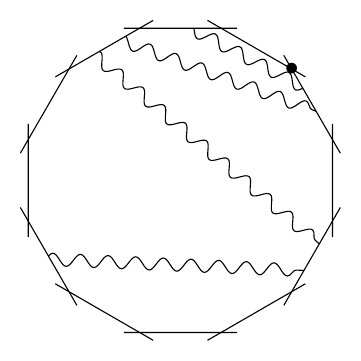
\begin{tikzpicture}[rotate=15]
\begin{scope}
\drawWLD{12}{2}
\drawprop{3}{2}{10}{2} % P
% number vertices a,a+1,b,b+1 for prop P

% clip these
\drawprop{3}{-2}{12}{-2}
\drawprop{2}{0}{12}{2}
\drawprop{6}{0}{10}{-2} % p1


\end{scope}
\end{tikzpicture}
\caption{Base step: if $P$ survives $n$ steps of the algorithm, there must be another propagator $p_1$ to its right on edge $(b,b+1)$.}
\label{fig:base step of alg induction}
\end{figure}

The propagator $p_1$ forms the base step for the following induction:

Suppose that $p_r$ is a propagator supported on $(i,i+1,m,m+1)$ and removed at step $m+1$ of the algorithm; we will show that there must also be a propagator $p_{r+1}$ supported on $(i',i'+1,m',m'+1)$ with $i \leq i'$ and $m \geq m'$, which is removed at step $m'+1$.  Since we can't have both $i' = i$ and $m'=m$, $p_{r+1}$ bounds a region containing strictly fewer vertices than $p_r$.

Notice that if we restrict our attention to the region bounded by $p_r$ and the edges of the diagram from $i$ to $m+1$, then propagators outside of this region can affect the algorithm only at vertices $i$, $i+1$.  (The starting vertex 1 lies outside this region, by assumption.)

Given a propagator $p_r$ supported on $(i,i+1,m,m+1)$ and removed at step $m+1$, we must also have a propagator $q$ to its right which is removed at step $m$ (``protecting'' $p_r$ at step $m$).  This splits into two cases:

\textbf{Case I}: If $q$ is supported on $(k,k+1,m-1,m)$ for some $k \geq i$, then $p_{r+1}:=q$  satisfies the conditions of the induction step.

\textbf{Case II}: Suppose $q$ is supported on $(k,k+1,m,m+1)$ for some $k$; since the diagram is admissible, we have $k > i$.  In particular, anything that happens at vertex $k+1$ is unaffected by propagators outside the region bounded by $p_r$, since $k+1 > i+1$.  But $q$ must survive until step $m$, so there must be another propagator $q'$ to the right of $q$, which protects $q$ at step $k+1$.  The admissibility of $W$ implies that $q'$ is supported on $(j,j+1,k,k+1)$ for some $j \geq i$, and we can take $p_{r+1}:=q'$.

\begin{figure}
\begin{tabular}{ccc}
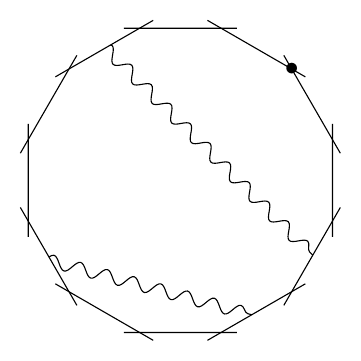
\begin{tikzpicture}[rotate=15]
\begin{scope}
\drawWLD{12}{2}
\drawprop{3}{0}{10}{0} % p_r
% number vertices i,i+1,m,m+1

%clip these
\drawprop{6}{0}{9}{0} % q
\end{scope}
\end{tikzpicture}

& \qquad \qquad &
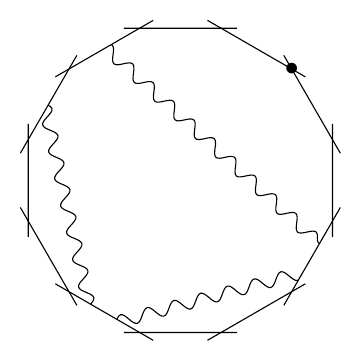
\begin{tikzpicture}[rotate=15]
\begin{scope}
\drawWLD{12}{2}
\drawprop{3}{0}{10}{2} % p_r
% number vertices i, i+1, m, m+1

\drawprop{7}{2}{10}{-2} %q
% vertices k,k+1, m,m+1

% clip this one
\drawprop{4}{0}{7}{-2} % q'
% vertices j,j+1,k, k+1

\end{scope}
\end{tikzpicture}
\\
Case I & & Case II
\end{tabular}

\caption{Inductive step: if propagator $q$ is removed at step $m$, then it lies on either edge $(m-1,m)$ (Case I) or $(m,m+1)$ (Case II).}
\label{fig: cases for inductive step, algorithm}
\end{figure}

By induction, we will eventually find a propagator on a region with 3 or fewer vertices, which is inadmissible.
\end{proof}


To prove that this algorithm gives the Grassmann necklace of the diagram we need two lemmas.

\begin{lem}\label{lem susama}
  \note{this lemma should be rephrased to be more in your language, it was just copied from the rank section, also it needs a cite or a proof}
  Given a WLD and a propagator $p$,  each covered vertex of $p$ is contributed to a non-empty cyclic interval in the Gra\ss mann necklace.
\end{lem}

\begin{lem}\label{lem basis as perm}
Let $W$ be an admissible Wilson loop diagram and let $\PP_W$ be the positroid associated to $W$.  A $k$-subset $J \in \binom{[n]}{k}$ is a basis for $\PP_W$ if and only if there is a set bijection between $J$ and the set of propagators of $W$ such that for each $j\in J$ the propagator associated to $j$ is supported on vertex $j$.
\end{lem}

\begin{proof}
\note{I don't know if you already have this in your previous papers or not; but it is important so I wanted to extract it as a lemma.  The proof of the next proposition originally contained the lines ``Recall from [ref] that a $k$-subset $J \in \binom{[n]}{k}$ is a basis for $\PP_W$ if and only if it has no subset $U \subseteq J$ such that $|U| > |Prop(U)|$.'' but I don't know what that ref is nor whether that ref would also prove this lemma.}
\end{proof}

\begin{prop}\label{res:alg gives GN}
The sequence of $k$-subsets obtained by applying Algorithm~\ref{alg:put GN on WLD} to an admissible diagram $W$ is exactly the Grassmann necklace of the positroid associated to $W$; specifically if we let  $I_i$ be the set of labels on edge $(i,i+1)$ then the sequence $\II = (I_1, \dots, I_n)$ is the Grassmann necklace of the positroid associated to $W$.
\end{prop}

\begin{proof}
Let $I_i$ be the set of labels on edge $(i,i+1)$; the sequence $\II = (I_1, \dots, I_n)$ is a Grassmann necklace if and only if $I_{i+1} \supseteq I_i \backslash \{i\}$ for all $i \in \{1, \dots, n\}$.


Suppose for a contradition that there exists an admissible diagram for which there exists an $i$ with $k\in I_{i\backslash\{i\}}$ and $k \not\in I_{i+1}$.  Fix $n$.  Let the triple $(W, i, k)$ be such a counterexample on $n$ vertices which is minimal with respect to the number of propagators. %, and among all those counterexamples on $n$ vertices with the same number of propagators, let $(W,i,k)$ be minimal with respect to the distance from $i$ to $k$ in the $\leq _i$ order.

If $i \not\in I_i$, then there are no propagators supported on $i$ at all.  In this case it is clear that applying Algorithm~\ref{alg:put GN on WLD} at vertex $i$ and vertex $i+1$ produces exactly the same result, i.e. $I_{i+1} = I_i$, and so $(W, i, k)$ is not a counterexample at all.

Now suppose that $i \in I_i$.  Let $p$ be the propagator which contributes $i$ to $I_i$.  Either $p$ has one end on the edge $(i-1, i)$ or it has one end on the edge $(i, i+1)$.  In both cases let $(b, b+1)$ be the edge with the other end of $p$.

\textbf{case I}:  Suppose $p$ has one end on $(i-1, i)$.  Then $p$ is not supported on $i+1$, so in building $I_{i+1}$ we will take the same propagators as in the construction of $I_i$ from vertices $i+1$ up to $b-1$, that is $I_{i+1} \cap \interval{i+1}{b-1} = I_{i} \cap \interval{i+1}{b-1}$.  Furthermore, by Lemma~\ref{lem susama}, in building $I_{i+1}$, it must be that $p$ is taken at vertex $b$, as otherwise $b$ would never be contributed by $p$.    Consequently, in building $I_{i+1}$, when at vertex $b$ no propagator still remaining is before $p$.  This is also true in building $I_i$ when at $b$ since the same propagators have been taken beforehand.  Additionally $k\geq_i b+1$.

Let $W'$ be the diagram obtained from $W$ by removing $p$ and all propagators under it in the sense of supported between $i+1$ and $b-1$.

By the above observations when we are in $W'$ at $b$ then we are in the same situation with respect to the remaining propagators as if we began at $i$ in $W$ and moved to $b$ following the algorithm; the propagators we took in the latter case are exactly the ones removed to build $W'$.  Similarly starting at $i+1$ in $W$ and moving to $b+1$ leaves us in the same situations with respect to the remaining propagators as beginning at $b+1$ in $W'$.  This gives the equations
\begin{align*}
  I_i^W \cap \interval{b}{i-1} & = I_b^{W'} \\
  I_{i+1}^W \cap \interval{b+1}{i-1} & = I_{b+1}^{W'}
\end{align*}
where the diagram is indicated in the superscript.
Thus we have $k\in I_b^{W'}\backslash\{b\}$ and $k\not\in I_{b+1}^{W'}$ contradicting the minimality of $(W, i, k)$.

\textbf{case II}: Suppose $p$ has one end on $(i, i+1)$.  Note that by definition $p$ is the propagator contributing $i$ to $I_i$ and so it must be the first propagator in $(i, i+1)$ and hence $p$ contributes $i+1$ to $I_{i+1}$.  Observe that $k\geq_i i+2$ since $i+1\in I_{i+1}$.

Let $W'$ be the diagram obtained from $W$ just by removing $p$.  Then
\begin{align*}
  I_i^W \backslash \{i\} & = I_{i+1}^{W'} \\
  I_{i+1}^W \backslash \{i+1\} & = I_{i+2}^{W'}
\end{align*}
since in both cases in $W'$ we are simply taking the remaining propagators in the same way as we would have in $W$ after taking $p$ for the previous vertex.  Since $k \neq i+1$, we have $k\in I_{i+1}^{W'}\backslash\{i+1\}$ but $k\not\in I_{i+2}^{W'}$ contradicting the minimiality of $(W, i, k)$

%If $i \not\in I_i$, then there are no propagators supported on $i$ at all.  In this case it is clear that applying Algorithm~\ref{alg:put GN on WLD} at vertex $i$ and vertex $i+1$ produces exactly the same result, i.e. $I_{i+1} = I_i$.
%
%Now suppose that $i \in I_i$.  Order $I_i$ and $I_{i+1}$ with respect to $\leq_{i+1}$; in particular, $i$ is the last term in $I_i$ with respect to this ordering.
%
%Let $p_1$ be the rightmost propagator supported on $i$, and suppose it is removed at step $a$ with respect to vertex $i+1$.  This is the first point at which $I_{i+1}$ can differ from $I_i$, i.e. we have $I_{i+1} \cap \interval{i+1}{a-1} = I_{i} \cap \interval{i+1}{a-1}$.  If $a \not\in I_i$, then $p_1$ is the only propagator supported on $a$ at step $a$ with respect to vertex $i+1$.  All remaining steps are unchanged and we conclude that $I_{i+1} = I_i \backslash \{i\} \cup \{a\}$.
%
%If $a \in I_i$, then at step $a$ with respect to vertex $i+1$ there must be another propagator $p_2$ which lies to the left of $p_1$.  We have $I_{i+1} \cap \interval{i+1}{a} = I_i \cap \interval{i+1}{a}$, and the next possible difference
%
%{\color{red}[argh]}
%
%Although there are many different subcases to consider, the idea is always the same: we look for the first entry where $I_{i+1}$ and $I_i \backslash \{i\}$ differ (with respect to $<_{i+1}$), and show that this is the only possible difference.
%
%The reader should keep in mind that due to Proposition~\ref{res:alg k labels}, the following process cannot double back on itself.
%
%\begin{enumerate}
%\item If $p_1$ contributes $k$ to $I_{i+1}$ and $k \in I_i$, then there is another propagator $p_2$ which was deleted at step $k$ with respect to vertex $i$, but now survives at step $k$ with respect to vertex $i+1$.  All intermediate steps of the algorithm are unchanged, so $I_{i+1}$ and $I_i \backslash \{i\}$ agree up to (and including) $k$.
%\item We now look at which label $p_2$ contributes in $I_{i+1}$, and apply the same argument.  Iterate this process until we find a propagator $p_r$ which is deleted at step $j$ with respect to vertex $i+1$, but $j \not\in I_i$.
%\item $j \not\in I_i$ implies that $p_r$ is the \textit{only} propagator supported on vertex $j$ at this step.  There is therefore no knock-on effect, and any remaining propagators in the diagram contribute the same label to both $I_i$ and $I_{i+1}$. We conclude that $I_{i+1} = I_i \backslash \{i\} \cup \{j\}$.
%\end{enumerate}

\medskip

We have shown that $\II$ is a Grassmann necklace; it remains to check that this Grassmann necklace defines the positroid $\PP_W$ associated to $W$.  We need to show that:
\begin{itemize}
\item For each $i \in \interval{1}{n}$, $I_i$ is a basis for $\PP_W$.
\item If $J$ is lexicographically smaller than $I_i$ with respect to $<_i$, then $J$ is not a basis for $\PP_W$.
\end{itemize}
The algorithm is pairing each $j \in I_i$ with a unique propagator supported on that vertex so by Lemma~\ref{lem basis as perm} $I_i$ is a basis for $\PP_W$.
%%Recall from [ref] that a $k$-subset $J \in \binom{[n]}{k}$ is a basis for $\PP_W$ if and only if it has no subset $U \subseteq J$ such that $|U| > |Prop(U)|$.  It is immediately clear from the construction that $I_i$ is a basis for each $i$: the algorithm is pairing each $j \in I_i$ with a unique propagator supported on that vertex, so $|Prop(U)| \geq U$ for all $U \subseteq I_i$.

%%If $\exists l \in J$ with $Prop(l) = \emptyset$ then $J$ is clearly not a basis, so suppose otherwise.  Write
%%\[I_i = [i_1 <_i i_2 <_i \dots <_i i_r <_i \dots <_i i_k], \quad J = [i_1 <_i i_2 <_i \dots <_i j_r <_i \dots <_i j_k],\]
%%so that $I_i$ and $J$ differ for the first time in the $r$th position.  Then
%%\[r-1 \geq |Prop(\{i_1, \dots, i_{r-1}\})| = |Prop(\{i_1, \dots, i_{r+1},j_r\})|,\]
%%If $|Prop(\{i_1, \dots, i_{r-1}|\}| = r-1$ then we are done; otherwise

Suppose we have $J$ such that $J$ is a basis and yet is lexicographically less than $I_i$ with respect to $<_i$.  By Lemma~\ref{lem basis as perm} there is a set bijection between $J$ and the propagators of $W$ such that the propagator associated to $j$ is supported on vertex $j$.  Choose one such bijection.  For a propagator $p$ of $W$ write $J(p)$ for the associated $j$ according to this bijection.  Similarly write $I_i(p)$ for the vertex assigned to $p$ by the algorithm.  Since $J$ is lexicographically smaller than $I_i$, the $<_i$-smallest element of the symmetric difference of $J$ and $I_i$ is some $j_0\in J$, $j_0 \not\in I_i$.

Let $p$ be the propagator such that $J(p)=j_0$.  Since $j_0\not\in I_i$ but $p$ is supported at $j_0$, then $I_i(p) <_i j_0$.  Thus the propagator $p$ has the following property: $I_i(p) <_i J(p)$ and $I_i\cap \interval{i}{I_i(p)} = J\cap \interval{i}{I_i(p)}$.  Call this property $A$.

{}From the previous paragraph we conclude that if we ever had a $J$ which is lexicographically less than $I_i$ and yet a basis of $\PP_W$ then there exists a propagator $p$ which has property $A$.

Finally, we will prove that whenever there is a propagator $p$ which has property $A$ then there is another propagator $r$ which also has property $A$ and for which $I_i(r) <_i I_i(p)$.  Since $I_i$ is finite this would lead to infinte regress and hence is impossible and thus there can be no such $J$ which will complete the proof of the proposition.

So suppose $p$ has property $A$.  The same vertices in $\interval{i}{I_i(p)}$ are in the image of the assignment from $J$ and the image of the assignment from $I_i$ so the same number of propagators are assigned to vertices in this interval by each assignment.  However $p$ is one of the propagators assigned to a vertex in this interval in $I_i$ but not in $J$.  Thus there exists a propagator $q$ for which $J(q)\in \interval{i}{I_i(p)}$ but $I_i(q) >_i I_i(p)$.  Therefore $J(q)<_i I_i(q)$ and  $I_i\cap \interval{i}{J(q)} = J\cap \interval{i}{J(q)}$.  This is analogous to property $A$ but with the roles of $J$ and $I_i$ switched.  Thus by the same argument we must have a propagator $r$ for which $I_i(r)\in \interval{i}{J(q)}$ but $J(r)>_i J(q)$.  Therefore $r$ has property $A$ which is what we wanted to prove.

\end{proof}

\subsection{Dimension of the Wilson Loop cells}

In \cite{reversingOh}, Agarwala and Fryer give an algorithm for passing from a Grassmann Necklace to a Le diagram. We use this algorithm here to pass from a Wilson loop diagram to its associated Le diagram. In this manner, we show that the positroid cell defined by a Wilson loop diagram has dimension $3|\cP|$. Maybe say something about Amplituhedra having $4k$ dimension, but this is not quite what we have, since we are ignoring one column.

When I speak of a \emph{WLD}, I mean one which satisfies your density hypothesis and other standard hypotheses.  When I speak of a propagator \emph{contributing} a vertex to an element of the Gra\ss mann\footnote{I suppose it is a bit of an affectation to use an eszett when writing in English, and actually the eszett is kind of ugly in this font, but since I've started to I'll stick with it for now but you certainly shouldn't feel obliged to do it too.} necklace I mean that according to the rule you guys have to build the Gra\ss mann necklace from the diagram by starting at a vertex and taking the clockwise-most covering propagator which hasn't already been taken, when a propagator is taken then it is contributing that vertex.  Also, I will be using your algorithm to convert the Gra\ss mann necklace into a Le diagram by non-intersecting paths.


We need four lemmas from stuff you guys have already figured out.  The first one is a corollary of your lemma characterizing intervals contributed by each covered vertex of a propagator.

The first lemma is Lemma~\ref{lem susama} and I moved it up to a previous section.

The second lemma is the fact that we understand uncovered vertices.  You probably see many ways to prove this from things you already know.  One would be to say that from your algorithm the column of the uncovered vertex simply plays no role.

\begin{lem}\label{lem uncovered}
  Let $D$ be a WLD with an uncovered vertex $i$.  Let $C$ be $D$ with $i$ removed.  Then the Le diagram of $D$ is the Le diagram of $C$ with an extra column of all $0$s inserted in the $|D|-i+1$th position from the left.
\end{lem}

The third lemma is Sian's result.

\begin{lem}\label{lem sian}
  Let $D$ be a WLD with all vertices covered by at least two propagators.  Then There exist two propagators in $D$ with the following properties.
  \begin{itemize}
  \item The first propagator goes from the edge $i$, $i+1$ to the edge $i+2$, $i+3$.
  \item The second propagator goes from the edge $i+2$, $i+3$ to the edge $i+4$, $i+5$
  \item No other propagator is on the edge $i+2$, $i+3$.
  \end{itemize}
\end{lem}

Actually the result I need is not exactly Sian's result and what I will actually use is her proof.  Thus I will use notation and definitions (including length of a propagator and the specific $p_i$ and $q_i$ construction from the proof) from her note without further discussion.  The result I will actually use will be that in place of the hypothesis that $D$ has all vertices covered by at least two propagators I have that all vertices are covered by at least 1 propagator and there are no propagators of length 3.

The fourth lemma is that we can rotate or reflect without changing the number of plusses.  The best way to see this is probably geometrically so I leave that up to you.

\begin{lem}\label{lem dihedral}
  If two WLDs differ by a dihedral transformation then their Le diagrams have same number of plusses.
\end{lem}

Now we're ready to go.

\subsubsection{Changes in Gra\ss mann necklaces for nice configurations}

Given a propagator $p$ in a WLD $D$, note that $p$ divides remaining propagators of $D$ into two sets depending on which side of $p$ they live.

\begin{lem}\label{lem good p}
  Let $D$ be a WLD with $n\geq 1$ propagators.  Then there is some dihedral transformation $D'$ of $D$ such that there is a propagator $p$ with the following properties.
  \begin{itemize}
  \item $p$ goes between the edge $i$, $i+1$ and the edge $n-1$, $n$ in $D'$.
  \item $i+2, \ldots, n-2$ are not covered by any propagators in $D'$ (which is trivially true if $\{i+1, \ldots, n-2\}=\varnothing$).
  \item Either $i+1$ in $D'$ is only covered by $p$, or $i+1$ is covered by exactly one other propagator $q$.
  \item If we are in the second case above then $q$ goes between the edge $j$, $j+1$ and the edge $i$, $i+1$ and $j+2, \ldots, i-1$ are not covered by any propagators.
  \end{itemize}
\end{lem}

\begin{proof}
  Since $n\geq 1$ the dual tree of $D$ has at least two vertices and so has at least two leaves.  Each edge going to a leaf of the dual tree corresponds to a propagator which has no other propagators on one side of it, so there is at least one such propagator in $D$.  There are two cases to consider.

  First suppose there is a propagator which has no other propagators on one side of it and for which one of its ends is on an edge with no other propagators.  Let this propagator be $p$.  Rotate and reflect $D$ as necessary so that the end of $p$ which does not share its edge comes first, then the side of $p$ with no other propagators, and then the other end of $p$ which is on edge $n-1$, $n$.  Call this WLD $D'$.  It is a straightforward check that the properties in the statement are satisfied with $i+1$ only covered by $p$.

  Next suppose there is no propagator which has no other propagators on one side of it and for which one of its ends is on an edge with no other propagators.  Let $C$ be $D$ with all uncovered vertices removed.  Suppose $C$ contains two propagators one of length 2 and one of length 3 with the length 2 propagator on the small side of the length 3 propagator.  Then we are in the case already considered because we can rotate and reflect $C$ so that these two propagators both have one end on the edge $|C|-1$,$|C|$, and have their other ends on the edge $|C|-2$, $|C|-3$ and the edge $|C|-3$, $|C|-4$, so taking the length 2 edge as $p$ we satisfy the properties of the statement, and this remains true in $D$.  Thus we now assume this does not occur, so in particular every propagator of length 3 in $C$ has no other propagators on its small side.  But then the middle vertex on this small side is uncovered contradicting the construction of $C$.  Thus $C$ has no propagators of size 3.

  The claim then is that in $C$ there must exist two propagators as in Lemma~\ref{lem sian}.  The proof of the claim follows by Sian's proof.  We do not have the hypothesis that all vertices are covered by at least two propagators, but this is only used in the proof of Lemma~\ref{lem sian} to force certain propagators (the $q_i$) to have length at least 4, so our this case we instead use that $C$ has no propagators of size $3$.

  Now rotate and flip $C$ so that the two propagators as in Lemma~\ref{lem sian} cover $\{|C|-5, \ldots, |C|\}$ and let $p$ be the propagator covering $\{|C|-3, \ldots, |C|\}$ and let $q$ be the other one.  Return to $D$ with a corresponding rotation and flip so that vertex $n$ in $D$ corresponds to vertex $|C|$ in $C$ and direction in the polygon is preserved.  Let this dihedral transformation of $D$ be $D'$.  Then the propagator $p$ satisfies the conditions of the statement with propagator $q$.
\end{proof}

Given a WLD $D$, $I_i^{D}$ denotes the $i$th Gra\ss mann necklace element corresponding to $D$.

\begin{lem}\label{lem I}
  Let $D$ be a WLD with $n\geq 1$ propagators and let $p$ be a propagator of $D$ so that the properties of Lemma~\ref{lem good p} are satisfied for $p$ in $D$ (that is $D$ is already appropriately transformed).  Furthermore suppose that that $p$ has length $2$, as does $q$ if we are in the case of Lemma~\ref{lem good p} involving $q$.  Let $C$ be $D$ with $p$ removed but no change in the vertices.  Then
  \begin{align*}
    I_1^{D} & = I_1^{C} \cup \{n-3\} \\
    I_n^{D} & = I_1^{C} \cup \{n\} \\
    I_{n-1}^{D} & = I_n^{C} \cup \{n-1\} \\
    I_{n-2}^{D} & =
    \begin{cases}
      I_{n-2}^{C}\cup \{n-2\} & \text{if $n-2\not\in I_{n-2}^{C}$} \\
      I_{n-2}^{C}\cup \{n-1\} & \text{if $n-2\in I_{n-2}^{C}$, $n-1\not\in I_{n-2}^{C}$} \\
      (I_{n}^{C} - \{n-5\})\cup \{n-1,n-2\} & \text{if $n-1, n-2\in I_{n-2}^{C}$}
    \end{cases} \\
    I_{k}^{D} & =
    \begin{cases}
      I_k^{C}\cup \{n-3\} & \text{if $n-3 \not\in I_k^{C}$}\\
      I_k^{C}\cup\{n-2\} & \text{if $n-3\in I_k^{C}$}
    \end{cases} \\
    & \text{for $1<k<n-2$}
  \end{align*}
\end{lem}

\begin{figure}
 % 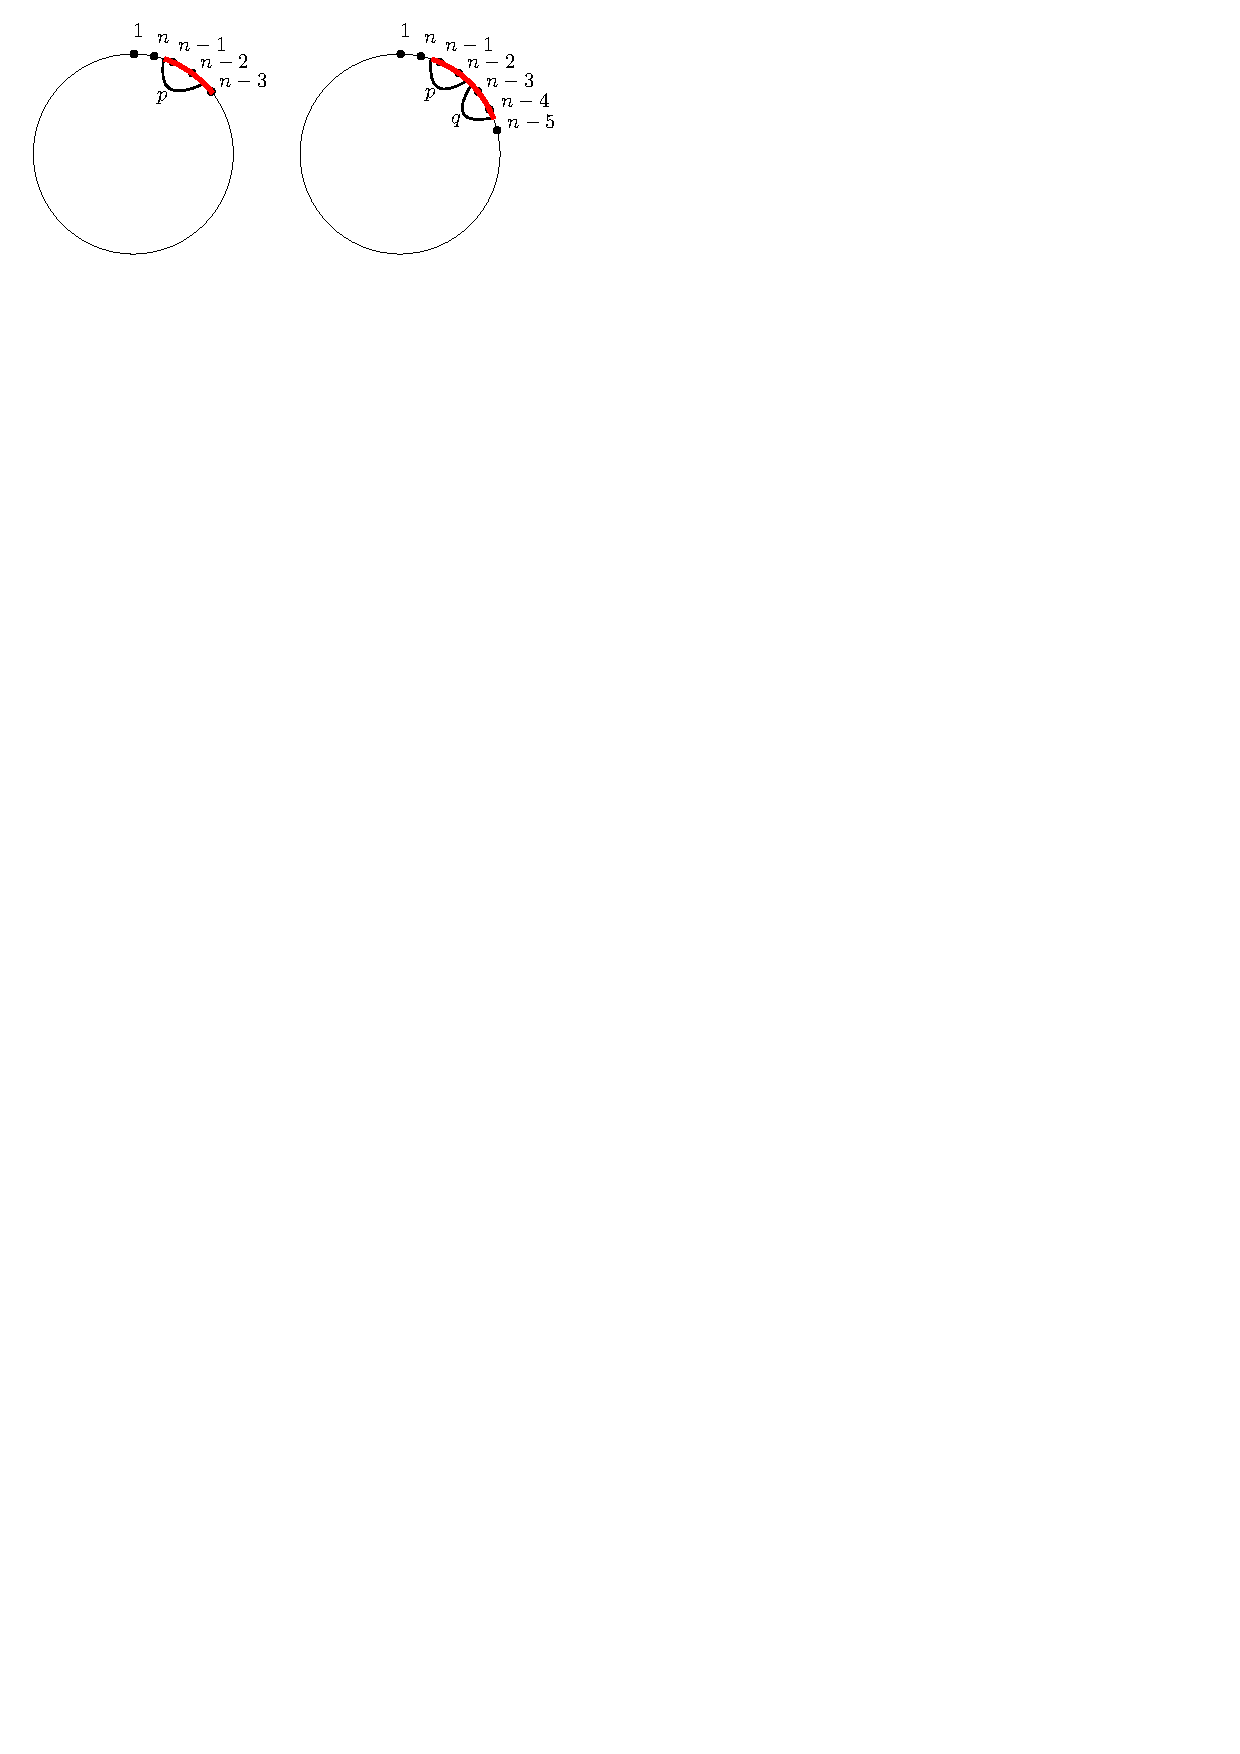
\includegraphics{specialp}
  \caption{The different possibilities for $D$ and $p$.  No other propagators can end in the fat red sections.  Other segments may have additional propagators ending in them.}\label{fig special p}
\end{figure}

\begin{proof}
  The two possible situations are illustrated in Figure~\ref{fig special p}.

  If $n-3\in I_1^{C}$ then $n-3\not\in I_1^{D}$, but then $p$ never contributes $n-3$ contradicting Lemma~\ref{lem susama}.  Thus $n-3\not\in I_1^{C}$ and so in building the Gra\ss mann necklace when we get to vertex $n-3$ any other covering propagators of $C$ have already been taken and so we can now take $p$.  Therefore $I_1^{D}= I_1^{C}\cup \{n-3\}$.

  In constructing $I_n^{D}$, first for vertex $n$ we take propagator $p$.  Then we are at vertex $1$ and precisely the propagators of $C$ remain.  Thus the rest of the construction will give $I_1^{C}$.  Therefore $I_n^{D} = I_1^{C}\cup \{n\}$.  Essentially the same reasoning gives $I_{n-1}^{D} = I_n^{C}\cup \{n-1\}$.

  Now consider $I_{n-2}^{D}$.  If $n-2\not\in I_{n-2}^{C}$ then at vertex $n-2$ we take $p$ and this does not affect the rest of the construction of $I_{n-2}^{C}$, so $I_{n-2}^{D} = I_{n-2}^{C}\cup \{n-2\}$.  An analogous argument takes care of the first case for $I_k^{D}$.  Suppose $n-2\in I_{n-2}^{C}$ but $n-1\not\in I_{n-2}^{C}$.  Then at vertex $n-2$ we take the same propagator in $C$ as in $D$ (in particular not $p$) because $p$ is the counterclockwisemost propagator covering $n-2$ and so the last propagator the algorithm would choose at this vertex, and by hypothesis $n-2$ is covered in $C$.  Howver, $n-1$ is untaken in $I_{n-2}^{C}$ so at this vertex we will take $p$ in $I_{n-2}^{D}$.  Following this, now that $p$ is out of the way without bumping any other propagators, the construction continues as in $I_{n-2}^{C}$.  Therefore $I_{n-2}^{D} = I_{n-2}^{C}\cup \{n-1\}$.  An analogous argument takes care of the case when we have $1<k<n-2$ and $n-3\in I_k^{C}$ but $n-2\not\in I_{k}^{C}$.  Furthermore, either $n-2$ is uncovered in $C$ or only $q$ covers $n-2$ in $C$ and $q$ is also the only propagator covering $n-3$.  Thus it is not possible for $n-3$ and $n-2$ to both be in $I_{k}^{C}$.  This means that all the cases for $I_k^{D}$ are now proved.

  The remaining case is when $n-1,n-2\in I_{n-2}^{C}$ for the construction of $I_{n-2}^{D}$.  We must then have a propagator $q$ as in the right hand side of Figure~\ref{fig special p}.  In the construction of $I_{n-2}^{D}$, at vertex $n-2$ we take propagator $q$, as in $I_{n-2}^{C}$.  Then at vertex $n-1$ we take propagator $p$ which is different from what occurs in $I_{n-2}^{C}$.  Next we are at vertex $n$ and propagators $p$ and $q$ have been taken.  Thus we are proceeding like $I_{n}^{C}$ but without propagator $q$.  Fortunately we can determine explicitely how propagator $q$ contributes to $I_{n}^{C}$.  By Lemma~\ref{lem susama} propagator $q$ contributes $n-5$ to $I_{n}^{C}$, and the only way this can occur is if all other propagators of $C$ were already taken by the time we got to vertex $n-5$.  Therefore $I_{n-2}^{D} = (I_{n}^{C} - \{n-5\}) \cup \{n-1, n-2\}$.  This covers all cases and hence completes the proof.
\end{proof}

\subsubsection{The number of plusses from Gra\ss mann necklaces in nice configurations}

\begin{lem}\label{lem shape}
  Let $C$ and $D$ be as in Lemma~\ref{lem I}.
  The shape of the Le diagram of $C$ can be built from left to right of the following blocks: a rectangle with 3 columns, one more column of the same length, a partition shape with at most as many rows as the rectangle.
  The shape of the Le diagram of $D$ can be built from left to right of the following blocks: a rectangle with 3 columns and one more row than the first rectangle of $C$, the same partition shape as in $C$.
\end{lem}

\begin{proof}
  $I_1$ determines the shape of the Le diagram.
  By Lemma~\ref{lem I}, $I_1^{D} = I_1^{C}\cup \{n-3\}$.  This implies that the right hand boundary of the shape of $C$ is the same as the right hand boundary of the shape of $D$ except that $D$ has one additional row of 3 boxes while $C$ has an additional column in the $n-3$ position, that is a new column fourth from the left.
\end{proof}

The shapes of the Le diagrams of $C$ and $D$ are illustrated in Figure~\ref{fig Le}.  The pieces of the Le diagrams will be called $\mathcal{A}$ and $\mathcal{B}$ in what follows, as in the figure.  Over the course of the next few lemmas we will prove that the plusses in the $\mathcal{B}$ parts of the Le diagrams of $C$ and $D$ are identical and the plusses in the $\mathcal{A}$ parts are very closely related.  When we speak of a plus in the Le diagram of $D$ being the same as in $D$ or vice versa, we mean that the plus' position in $\mathcal{A}$ or $\mathcal{B}$ is the same.  Because of the column insertion the absolute indices may differ.

\begin{figure}
%  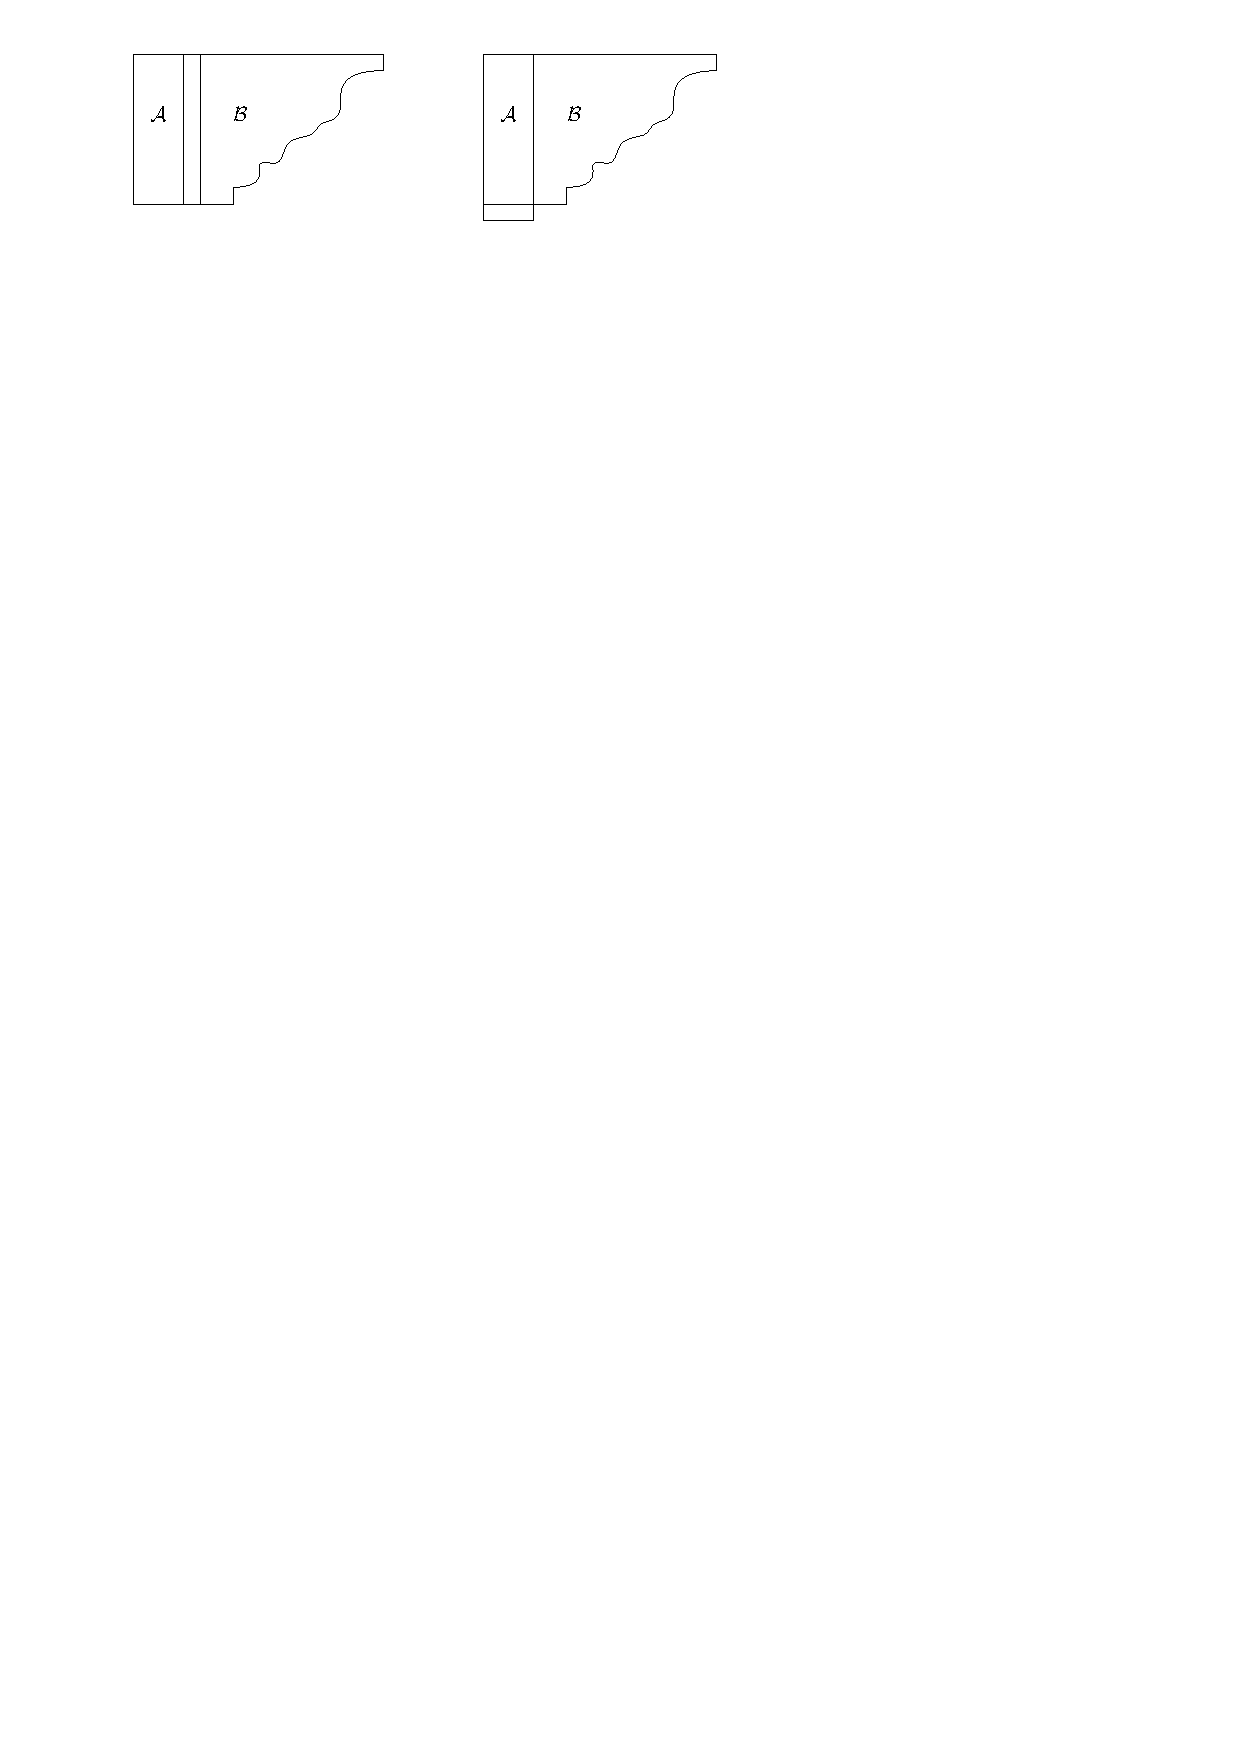
\includegraphics{Le_diagrams}
  \caption{Le diagrams for $C$ (left) and $D$ (right).}\label{fig Le}
\end{figure}

Suppose we are following the Gra\ss mann necklace to Le diagram algorithm, and we put a plus in a box because of a path from vertical boundary edge $i$ to bottom boundary edge $j$.  Then say this plus is in the $i\rightarrow j$ position.

\begin{lem}\label{lem n and n-1}
  Let $C$ and $D$ be as in Lemma~\ref{lem I}.
  The $I_n^{D}$ and $I_{n-1}^{D}$ elements of the Gra\ss mann necklace of $D$ give all the same plusses as $I_n^{C}$ along with plusses in the leftmost two boxes of the bottom row of the Le diagram of $D$.
\end{lem}

\begin{proof}
  By Lemma~\ref{lem I} $I_n^{D}= I_1^{C} \cup \{n\}$, so by the Gra\ss mann necklace to Le diagram algorithm the only plus this builds in the Le diagram of $D$ is  the one in the $n-3\rightarrow n$ position, that is in the leftmost box of the bottom row.

  Also by Lemma~\ref{lem I} $I_{n-1}^{D} = I_n^{C} \cup \{n-1\}$.  Additionally $n-3\not\in I_{n}^{C}$ since if it were then $n-3$ would also be in $I_1^{C}$ and hence propagator $p$ could not contribute $n-3$ to $I_1^{D}$ in contradiction to Lemma~\ref{lem susama}.  Similarly $n-1, n-2\not\in I_n^{C}$.  Thus the paths putting the plusses in from $I_n^{C}$ lie completely in $\mathcal{B}$ or take some vertical boundary edge $>n-3$ to $n$.   Now view these paths in the Le diagram of $D$ and note that the path $n-3\rightarrow n-1$ is compatible, and so these paths together build the plusses that $I_{n-1}^{D}$ contributes.  That is, we get all the plusses from $I_{n}^{C}$ along with a $n-3\rightarrow n-1$ plus, that is a plus in the second to the right box of the bottom row.
\end{proof}

\begin{lem}\label{lem n-2 good}
  Let $C$ and $D$ be as in Lemma~\ref{lem I} with $n-2 \not\in I_{n-2}^{C}$.

  The $I_{n-2}^{D}$ element of the Gra\ss mann necklace of $D$ gives
  an $n-3\rightarrow n-2$ plus and
  all the $I_{n-1}^{C}=I_{n-2}^{C}$ plusses.
\end{lem}

\begin{proof}
  If $n-2\not\in I_{n-2}^{C}$ then $I_{n-1}^{C}=I_{n-2}^{C}$ and by Lemma~\ref{lem I} $I_{n-2}^{D} = I_{n-1}^{C} \cup \{n-2\}$.  Note that $n-3\not\in I_{n-2}^{C}$ by Lemma~\ref{lem susama}.  Therefore the paths for $I_{n-2}^{D}$ are the paths for $I_{n-1}^{C}$ along with the $n-3\rightarrow n-2$ path.  This gives the statement of the lemma.

\end{proof}

\begin{lem}\label{lem n-2 bad}
  Let $C$ and $D$ be as in Lemma~\ref{lem I} with $n-2,n-1 \in I_{n-2}^{C}$.

  The $I_{n-2}^{D}$ and $I_{n-3}^{D}$ elements of the Gra\ss mann necklace of $D$ gives the following plusses:
  \begin{itemize}
  \item An $n-3\rightarrow n-2$ plus and an $n-5\rightarrow n-1$ plus.
  \item All the $I_{n-1}^{C}$ plusses.
  \item $I_{n-2}^{C}$ gives an $n-5\rightarrow n-2$ plus and no other term in the Gra\ss mann necklace of $C$ gives a plus in this column.  This $+$ does not appear in $D$ from $I_{n-2}^{D}$ but an $n-5\rightarrow n-1$ plus does instead.
  \item All other plusses of $I_{n-2}^{C}$.
  \item $I_{n-3}^{C}$ gives a plus in the $n-3$ column.  This $+$ is shifted over into the $n-2$ column in $D$.
  \item All other plusses of $I_{n-3}^{C}$.
  \end{itemize}
  Furthermore, no element of the Gra\ss mann necklace of $C$ gives an $n-5\rightarrow n-1$ plus.
\end{lem}

\begin{proof}
  By Lemma~\ref{lem I} $I_{n-2}^{D}= (I_{n}^{C} - \{n-5\})\cup \{n-1,n-2\}$.  Also, by the location of $q$ in the WLD,  $n-2\not\in I_{n-3}^{C}$ and and $n-5$ is the index of the lowest vertical edge in $\mathcal{B}$.  Thus this section of the Gra\ss mann necklace of $C$ looks like
  \begin{equation}\label{eq necklace}
  I_{n-3}^{C} \underset{\substack{n-3\text{ out}\\n-2\text{ in}}}{\rightarrow} I_{n-2}^{C} \underset{\substack{n-2\text{ out}\\n-5\text{ in}}}{\rightarrow} I_{n-1}^{C} \underset{\substack{n-1\text{ out}\\\text{something in}}}{\rightarrow} I_{n}^{C} \underset{\substack{n \text{ out}\\\text{something in}}}{\rightarrow} I_1^{C}
  \end{equation}
  where the first ``something'' is either $n$ or an element of $I_1^{C}$ and the second ``something'' is an element of $I_1^{C}$.  Additionally all elements not explicitly mentioned must be in $I_1^{C}$ as they remain unchanged through this portion of the necklace.

  Using this information now determine the symmetric difference of $I_{n-2}^{C}$ and $I_1^{C}$: $n-1, n-2$ and possibly $n$ are in $I_{n-2}^{C}$ but not in $I_1^{C}$.  $n-5$ is in $I_1^{C}$ as are at least one and at most two other elements.  If there is one such element call it $a$.  If there are two call them $a$ and $b$ with $a>b$.  This means that the plusses in the Le diagram of $C$ coming from $I_{n-2}^{C}$ are as in the first part of Figure~\ref{fig messy}.  Stepping to $I_{n-1}^{C}$ simply removes the $n-5\rightarrow n-2$ path, see the second part of Figure~\ref{fig messy}.

  \begin{figure}
 %   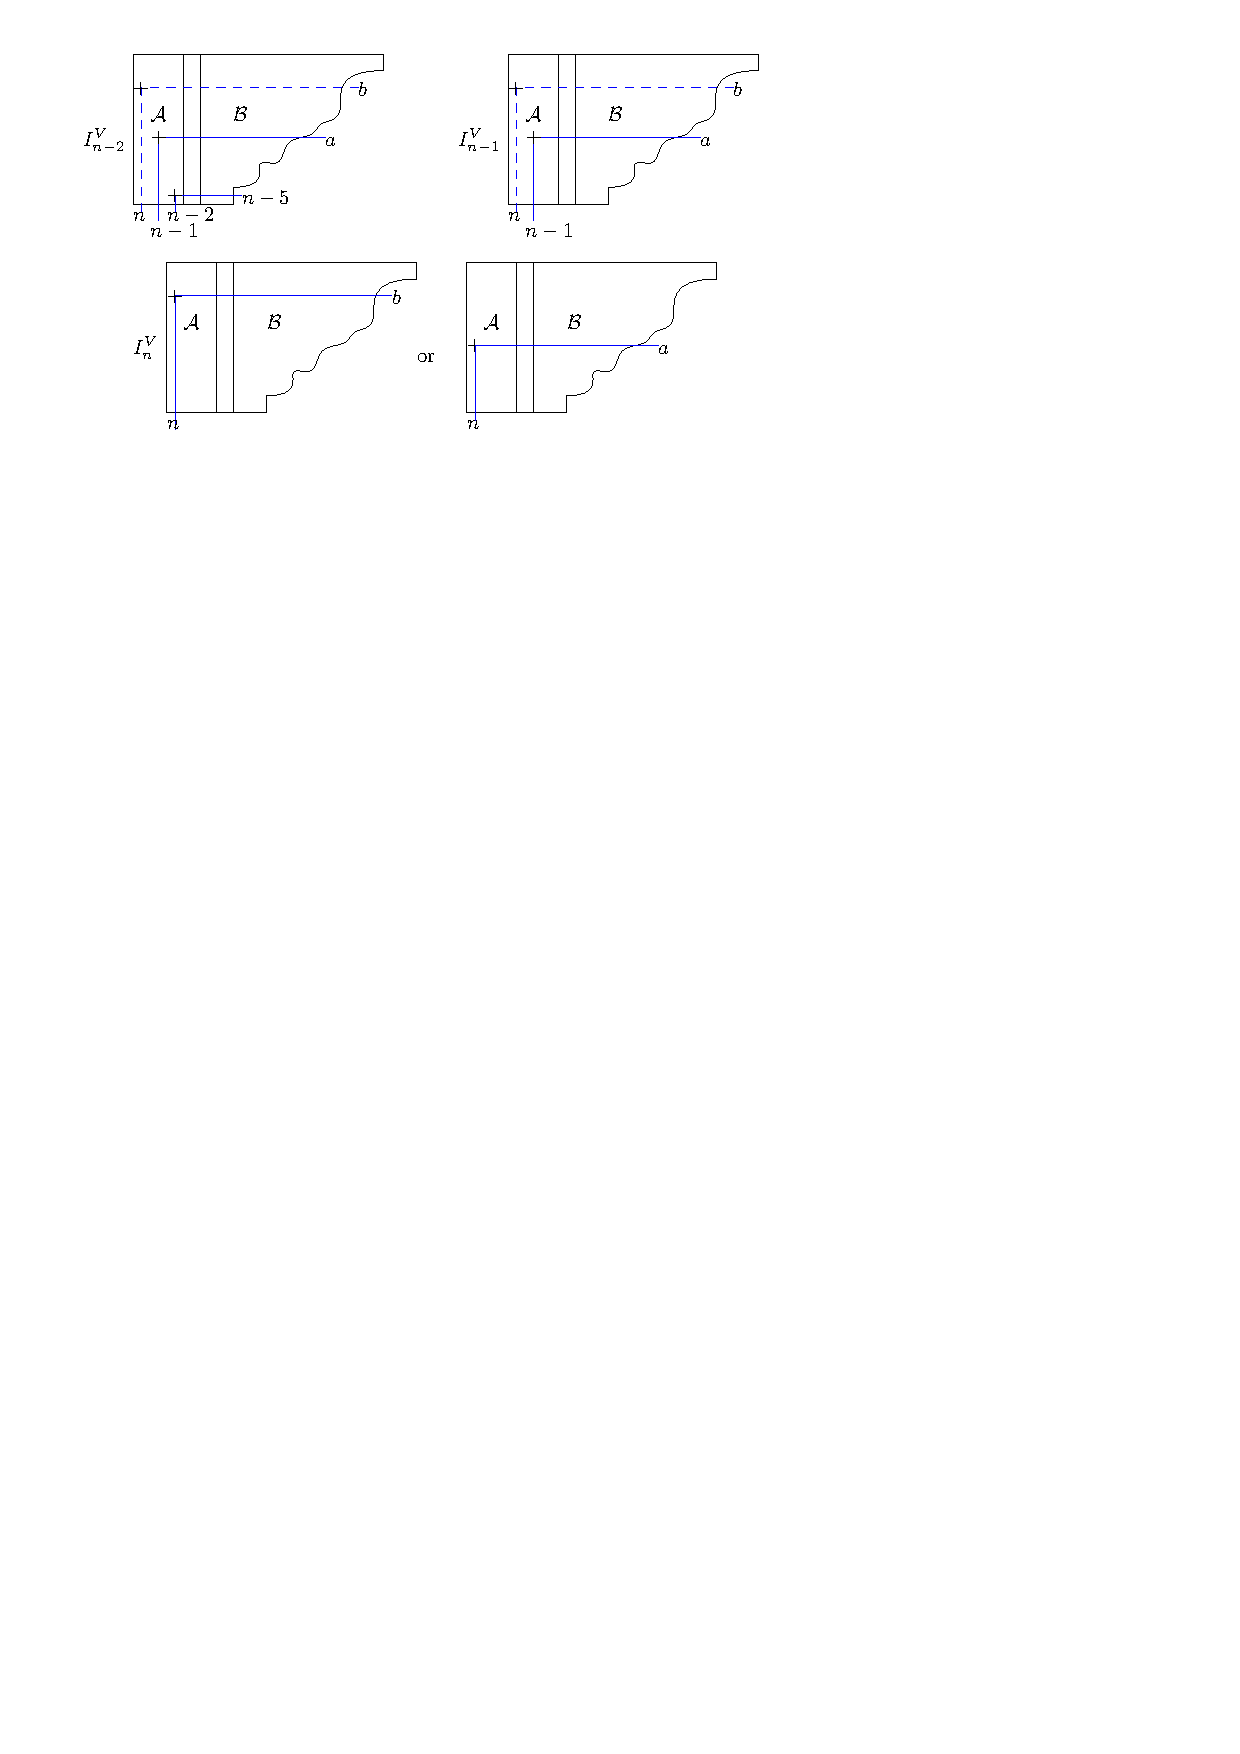
\includegraphics{messy}
    \caption{Plusses coming from $I_{n-2}^{C}$ (top left),  $I_{n-1}^{C}$ (top right) and $I_{n}^{C}$ bottom when $n-1, n-2\in I_{n-1}^{C}$.  The blue lines are the non-intersecting paths.  The dashed blue lines may or may not appear, but if one appears then they both do.}\label{fig messy}
  \end{figure}

  Stepping to $I_{n}^{C}$, $n-1$ is taken out and either $n$ is put in if it was not there before, or one of $a$ or $b$ is put in and hence no longer available as a right end for a path.  This gives two possible configurations illustrated in the bottom two parts of Figure~\ref{fig messy}.

  Now we know that $I_{n-2}^{D}  = (I_{n}^{C} - \{n-5\})\cup \{n-1,n-2\}$ so the paths for building plusses from $I_{n-2}^{D}$ go from the set $\{n-5, n-3\}$ along with whichever of $a$ and $b$ is not in $I_{n}^{C}$ to $\{n-2, n-1, n\}$.  This means that we get plusses as in Figure~\ref{fig messyD} where the left and right cases correspond to the left and right cases in the bottom parts of Figure~\ref{fig messy}

  \begin{figure}
    % 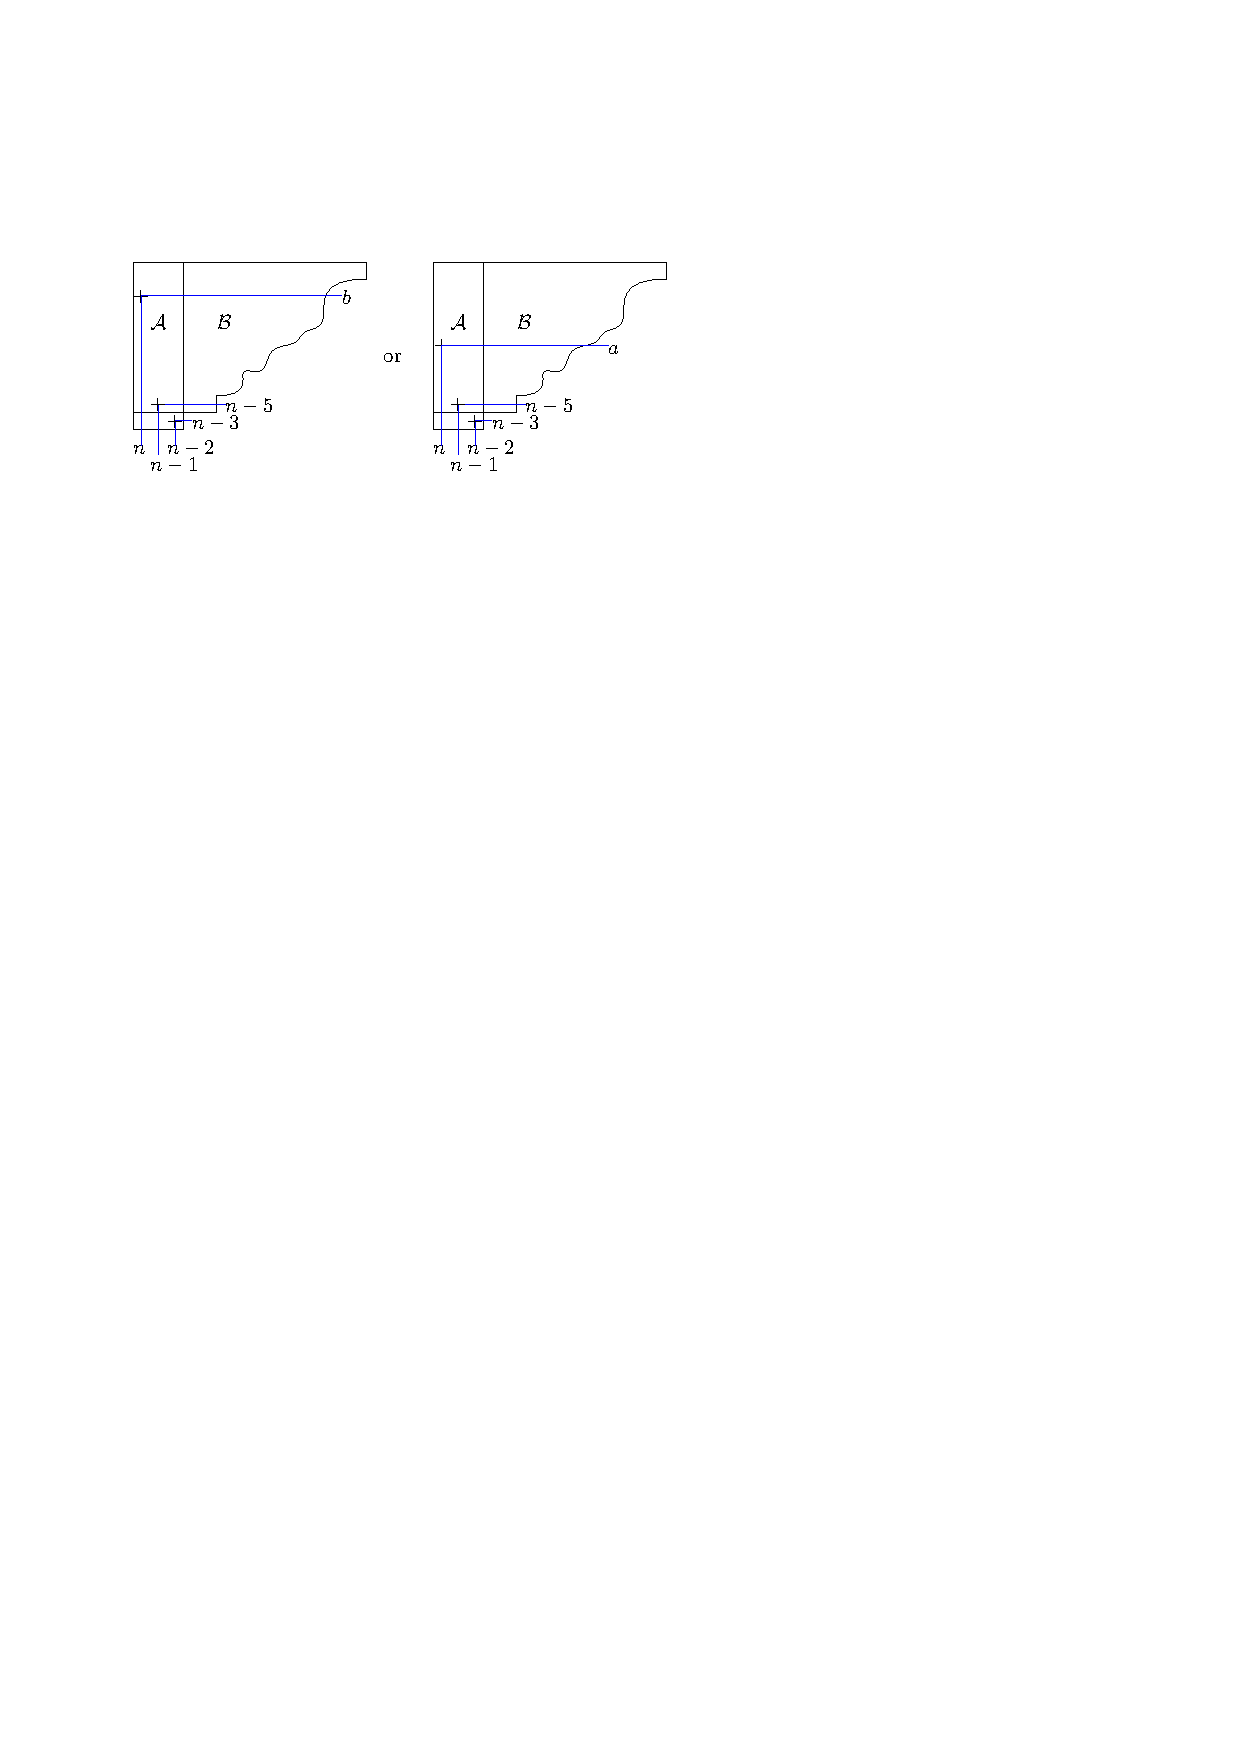
\includegraphics{messyD}
    \caption{Plusses coming from $I_{n-2}^{D}$.}\label{fig messyD}
  \end{figure}

  This proves the first item of statement of the lemma.

  Now consider $I_{n-3}^{C}$.  By \eqref{eq necklace} $I_{n-3}^{C}$ contributes the same plusses as $I_{n_2}^{C}$ except that it contributes an $n-5\rightarrow n-3$ plus in place of the $n-5\rightarrow n-2$ plus.  Also, we have $n-3\in I_{n-3}^{C}$ be the location of $q$ and so $I_{k}^{D} = I_k^{C}\cup\{n-2\}$.  Thus the paths for $I^{D}_{n-3}$ are the same as for $I^{C}_{n-3}$ except that the path that did go to $n-3$ now goes to $n-2$.  This cannot conflict with another path since \eqref{eq necklace} shows that $n-2$ only appears in $I_{n-2}^{C}$ among the necklace elements of $C$.

  Also note that $I_{n-3}^{C}, I_{n-2}^{C}$, and $I_{n-1}^{C}$ share their plusses outside of the $n-3$ and $n-2$ columns.  This proves the remaining statements of the lemma except the furthermore.

  Finally, suppose there were a $n-5\rightarrow n-1$ plus in the Le diagram of $C$.  By the algorithm, it would have to come when $n-5 \not\in I_j^{C}$.  By \eqref{eq necklace} this means that it would have to come from $I_{n-4}^{C}$, $I_{n-3}^{C}$, or $I_{n-2}^{C}$. The analysis above shows it does not come from $I_{n-3}^{C}$ or $I_{n-2}^{C}$.   Now, $n-4\in I_{n-4}^{C}$ by the location of $q$ and so $I_{n-4}^{C}$ must give an $n-5\rightarrow n-4$ plus and so cannot give an $n-5\rightarrow n-1$ plus.

\end{proof}


\begin{lem}\label{lem other k}
  Let $C$ and $D$ be as in Lemma~\ref{lem I} and take $1<k<n-2$.  Suppose that if $n-2\in I_{n-2}^{C}$ then also $n-1\in I_{n-2}^{C}$.
  The $I_k^{D}$ element of the Gra\ss mann necklace of $D$ gives the same plusses as $I_{k}^{C}$ except that if there is a plus in the $n-3$ column for $I_{k}^{C}$ then this plus is shifted into the $n-2$ column and no plus was already in that location.
\end{lem}

\begin{proof}
  If $n-3\not\in I_{k}^{C}$ then by Lemma~\ref{lem I} $I_{k}^{D} = I_k^{C}\cup \{n-3\}$.  Then since $n-3$ is the largest element of $I_1^{D}$ this transformation leaves the disjoint paths unchanged and so the plusses carry over from $C$ to $D$ directly.

  If $n-3\in I_{k}^{C}$ then by Lemma~\ref{lem I} $I_{k}^{D} = I_k^{C}\cup \{n-2\}$.  If $n-2$ is not covered in $C$ then certainly no pluses appear in the $n-2$ column of the Le diagram of $C$.  If $n-2$ is covered in $C$ then by hypothesis so is $n-1$ and so we satisfy the hypotheses of Lemma~\ref{lem n-2 bad}.  Thus the only necklace element of $C$ containing $n-2$ is $I_{n-2}^{C}$ and this particular plus is not contributed to the Le diagram of $D$ by $I_{n-2}^{D}$.

  {}From $I_{k}^{C}$ there is a path from some vertical edge to the bottom edge $n-3$.  In $I_{k}^{D}$, $n-3$ is a vertical edge with no path and instead there must be a path to $n-2$.  By the previous paragraph no other path can end in $n-2$, so shifting the path that did go to $n-3$ to go to $n-2$ while leaving the others the same maintains non-crossingness and so must be the paths for $I_{k}^{D}$.  Thus the plus in the $n-3$ column for $C$ is shifted into the $n-2$ column, where there was no plus before, and no other plusses are changed.
\end{proof}

\begin{thm}
  The number of plusses in the Le diagram of a WLD is three times the number of propagators.
\end{thm}

\begin{proof}
  The proof is by induction on the number of propagators.

  First note that a WLD $D$ with one propagator covering vertices $i<j<k<\ell$ has Le diagram a single row with $|D|-i$ boxes.  Labelling them from left to right by $|D|, \ldots, |D|-i+1$, by the algorithm there are plusses in the $j$, $k$, and $\ell$ positions.

  Now consider WLDs with $k>1$ propagators.  By Lemma~\ref{lem uncovered} it suffices to prove the result for WLDs with $k$ propagators and no uncovered vertices.  By Lemma~\ref{lem dihedral} it suffices to prove the result for at least one WLD from each dihedral orbit.  Take a WLD diagram $D$ with $k$ propagators.  Make a dihedral transformation of $D$ if necessary so that $D$ has a propagator $p$ with the properties in Lemma~\ref{lem good p} relative to $D$.  If $n-1$ is only covered by $p$ but $n-2$ is covered by at least one other propagator, then flip $D$ on the line perpendicular to the edge from $n-2$ to $n-1$.  This will be our $D$ for the rest of the proof.

  Let $C$ be $D$ with $p$ removed but no change in the vertices.  Note that if $n-2$ is covered in $C$ then so is $n-1$ by the end of the previous paragraph and so if $n-2$ is covered in $C$ then the hypotheses of Lemma~\ref{lem n-2 bad} are satisfied.

  {}From Lemma~\ref{lem shape} we know how the shapes of the Le diagrams of $C$ and $D$ relate; let $\mathcal{A}$ and $\mathcal{B}$ be as described after that lemma.  Lemmas~\ref{lem n and n-1}, \ref{lem n-2 good}, and \ref{lem n-2 bad} tell us that the three boxes of the bottom row of the Le diagram of $D$ each have a plus.  Lemmas~\ref{lem n and n-1}, \ref{lem n-2 good}, \ref{lem n-2 bad}, and \ref{lem other k} show that there is a bijection between the plusses of the Le diagram of $C$ and the plusses of the Le diagram of $D$ that are not in the bottom row which can be described as follows.
  \begin{itemize}
  \item Plusses from $\mathcal{B}$ for $C$ maintain their positions in $\mathcal{B}$ for $D$.
  \item Plusses from the first two columns (the $n$ and the $n-1$ columns) of $\mathcal{A}$ for $C$ maintain their positions in $\mathcal{A}$ for $D$.
  \item If there is a plus in the $n-2$ column of $\mathcal{A}$ in  then Lemma~\ref{lem n-2 bad} applies, so there is exactly one such plus.  This plus maps to the $n-5\rightarrow n-1$ plus for $D$.
  \item The plusses in the $n-3$ column for $C$ shift over to the third column (the $n-2$ column) of $\mathcal{A}$ in $D$.
  \end{itemize}
  This map is clearly reversible and hence bijective except possibly for the $n-5\rightarrow n-1$ plus for $D$.   If the Le diagram of $D$ has an $n-5\rightarrow n-1$ plus then look at the Le diagram for $C$.  If the Le diagram for $C$ has a plus in the $n-2$ column then Lemma~\ref{lem n-2 bad} applies and so there is no $n-5\rightarrow n-1$ plus in the Le diagram of $C$ and the $n-5\rightarrow n-1$ plus of $D$ can be uniquely mapped to the plus in the $n-2$ column of the Le diagram of $C$.  If the Le diagram for $C$ has no plus in the $n-2$ column, then leave the $n-5\rightarrow n-1$ plus where it is in moving back to $C$.  This reverses the map.

  From all of this we get that the number of plusses in the Le diagram for $D$ is three more than the number of plusses in the Le diagram for $C$.  Applying induction completes the proof.
\end{proof}


{\color{red}Maybe proved that inadmissible diagrams, while they correspond to matroids, can't be mapped to the positroids of the correct dimension? }

\section{Poles of Wilson Loop Integrals}

Put some exposition here about Theorem~\ref{thm denom}.

We can also use the ideas of the above constructions to understand the denominator of the integral $I(W)$.

\begin{algorithm}\label{alg WLD to denom via GN}
Let $W$ be a Wilson loop diagram with $n$ vertices.  Let $C(W)$ be the matrix \hlfix{which has some actual name and a ref to where you define it}.
\begin{itemize}
  \item For each $i \in \interval{1}{n}$, we construct a factor $r_i$ as follows
    \begin{itemize}
      \item Use Algorithm~\ref{alg:put GN on WLD} to obtain a bijection between the propagators and the $i-1$st Grassmann necklace element, $I_{i-1}$.  Write $I_{i-1}(p)$ for the vertex associated to propagator $p$ under this bijection.
      \item Use Algorithm~\ref{alg:put GN on WLD} to obtain a bijection between the propagators and the $i$th Grassmann necklace element, $I_{i}$.  Write $I_{i}(p)$ for the vertex associated to propagator $p$ under this bijection.
      \item Let $S_i$ be the set of propagators $p$ such that $I_{i-1}(p) \neq I_{i}(p)$.
      \item $\Delta_{I_i}$ is the determinant of the $k \times k$ minor of $C(W)$ indicated by $I_i$.
      \item Let $r_i$ be $\Delta_{I_i}$ with all variables from rows associated to $p\not\in S_i$ set to $1$.
    \end{itemize}
  \item $R = \prod_{i=1}^n r_i$.
\end{itemize}
\end{algorithm}

\begin{prop}\label{prop alg gives rad}
  With notation as in Algorithm~\ref{alg WLD to denom via GN} we have the following:
  \begin{enumerate}
    \item Each $\Delta_{I_i}$ is homogeneous.
    \item Each $\Delta_{I_i}$ splits into linear and quadratic factors.  All linear factors of  $\Delta_{I_i}$ are single variables and all quadratic factors are $2\times 2$ determinants of single variables.
    \item Quadratic factors in $r_i$ arise precisely when propagators $p$ and $q$ are supported on a common edge $(a,b)$ and $I_i(p)=a$, $I_i(q)=b$.
    \item $r_i$ divides $\Delta_{I_i}$.
    \item $R$ is the radical of $\prod_{i=1}^{n}\Delta_{I_i}$.
  \end{enumerate}
\end{prop}

\begin{proof}
\begin{enumerate}
    \item The nonzero entries of $C(W)$ are independent indeterminates and so every $i\times i$ minor of $C(W)$ is homogeneous of degree $i$ or is $0$.  Thus each $\Delta_{I_i}$ is homogeneous.
    \item Using the expression for the determinant as a sum over permutations we see that $\Delta_{I_i}$ is a sum over bijections between $I_i$ and $\mathcal{P}$.  The nonzero terms in this sum are precisely those bijections such that each propagator is associated to one of its supporting vertices in $I_i$, since only those locations in $C(W)$ are nonzero.  Since the nonzero entries of $C(W)$ are independent there can be no cancellation between terms in this expansion.

Suppose $\Delta_{I_i}$ has an irreducible factor $f$.  Let $\mathcal{P}'$ be the set of propagators which contribute a variable to $f$ and let $J$ be the set of vertices which contribute a variable to $f$.

The first claim is that the minor of $C(W)$ associated to $\mathcal{P}'$ and $J$ is precisely $f$.

Proof of claim: By the structure of determinants $\Delta_{I_i} = fg$ where $g$ involves only variables associated to propagators not in $\mathcal{P}'$ and associated to vertices not in $J$.  Expanding out $fg$, then, we get a signed sum of monomials where in each monomial $f$ contributes those variables associated both to a propagator in $\mathcal{P}'$ and to a vertex in $J$ and $g$ contributes those variables associated both to a propagator not in $\mathcal{P}'$ and to a vertex not in $J$ and no other variables appear.  Since there is no cancellation between terms, this means that $\Delta_{I_i}$ contains no other variables.  Therefore $\Delta_{I_i}$ is the same as the determinant of the matrix obtained by taking the submatrix of $C(W)$ which gave $\Delta_{I_i}$ and setting all these other variables to $0$.  This new matrix is, up to permutations of rows and columns, a block matrix with one block for $\mathcal{P}'$ and $J$ and the other block for the complements.  Thus its determinant, and hence also $\Delta_{I_i}$, is the product of the minors for these two blocks.  By which variables appear, these two factors are also $f$ and $g$ and so in particular $f$ is the minor of $C(W)$ associated to $\mathcal{P}'$ and $J$.

A consequence of this claim is that every linear factor of $\Delta_{I_i}$ is a $1\times 1$ minor of $C(W)$, hence is a single variable, and every irreducible quadratic factor of $\Delta_{I_i}$ is a $2\times 2$ minor of $C(W)$, hence is a $2\times 2$ determinant of single variables.

The final thing to prove for this item is that there are no irreducible factors $f$ of degree 3 or more.  Now suppose for a contradiction that $f$ has degree $\geq 3$. Note that by removing the propagators which do not contribute to $f$ and changing $i$ to be the first vertex which contributes to $f$ we obtain a different admissible diagram for which $f=\Delta_{I_i}$ and $i\in I_i$.  Showing that this different admissible diagram gives a contradiction is sufficient, and so we may assume that $W$ has $\Delta_{I_i}$ irreducible of degree 3 or more and $i\in I_i$.

Let $p$ be the propagator such that $I_i(p) = i$. There are two cases to consider.  

\textbf{Case I}: Suppose $p$ is supported on $(i-1, i, m, m+1)$ for some $m >_i i$.  Then $I_{i+1}(p) = m$ by Lemma~\ref{lem susama}.  Call the propagators which appear before $p$ is closed the propagators inside $p$. \note{It might be nice to have general language for this inside/outside idea.  What do you think.}  The construction of $I_{i+1}$ begins as for $I_i$ after the first step; they can only differ once $p$ contributes to $I_{i+1}$.  Thus if a propagator contributes $m$ in $I_i$ then it cannot be a propagator inside $p$ (nor $p$ itself).  Let $S$ be the set of propagators inside $p$ along with $p$ itself.  Two things can now happen; if neither $m$ nor $m+1$ appear in $I_i$ then the only vertex in the support of $p$ in $I_i$ is $i$, and so the row of $p$ in the matrix of $\Delta_{I_i}$ has only one nonzero entry; hence $\Delta_{I_i}$ has a linear factor which is a contradiction.  The other think which can happen is that at least one of $m$ and $m+1$ is in $I_i$.  However, all the propagators in $S$ are mapped by the bijection of $I_{i}$ to vertices strictly before $m$ so the matrix giving $\Delta_{I_i}$ has the form
\[
\begin{bmatrix} A & B \\ 0 & C\end{bmatrix}
\]
where $A$ is the matrix for the propagators in $S$ and the vertices in $I_i(S)$ which is square of size $|S|\times |S|$. No other propagators can be supported on these vertices since all other propagators are outside of $p$ and $p$ is the first propagator supported at $i$.  This explains the zero block.  Therefore $\Delta_{I_i} = \det A \det C$ and both factors are nontrivial since $m$ appears in $I_i$.  This contradicts the irreducibility of $\Delta_{I_i}$.

\textbf{Case II}:

\note{I am here}

\note{Proving that there are no factors larger than quadratic has been much tougher than I anticipated.  Maybe you have a better idea of how to approach it.}

    \item
    \item
    \item
  \end{enumerate}
\end{proof}


\begin{thm}\label{thm denom}
Given any admissible Wilson loop diagram $W$, let $GN(W) = \{I_1, \ldots I_n\}$ be the associated Grasmann necklace. Then the denominator of the integral $I(W)$ is the \hlfix{find correct word for this} is the minimal polynomial of $\prod_{i=1}^n \Delta_{I_i}$, where $\Delta_{I_i}$ is the determinant of the $k \times k$ minor indicated by $I_i$.
\end{thm}

\begin{proof}
In view of Proposition~\ref{prop alg gives rad} it remains to prove that the $R$ of Algorithm~\ref{alg WLD to denom via GN} is $R(W)$, the denominator of the integral $I(W)$.

\note{I don't want to write the rest of this right now because we need to somewhere (probably much earlier in the document) define $R(W)$ and exactly how we do so makes a difference.  The definition I would most like is if we define it as the product of the prop together and prop to vertex limits, if we define it some other way I'll probably want a lemma to get to that formulation.}

\end{proof}

\end{document}
